\documentclass{llncs}
\usepackage{amsmath}
\usepackage{amssymb}
\usepackage{float}
\usepackage[urlcolor=blue,linkcolor=black,colorlinks=true]{hyperref}
\hypersetup{
  pdftitle = {A Novel Approach to Detecting DNS Tunnels Using Throughput Estimation},
  pdfkeywords = {},
  pdfauthor = {Michael Himbeault and Jacky Baltes}
}
\usepackage[dvips]{graphicx}
\usepackage{lscape}
\usepackage{subfigure}
\usepackage{makeidx}  % allows for indexgeneration

\begin{document}

%\frontmatter
%\bibliographystyle{abbrv}
\title{A Novel Approach to Detecting DNS Tunnels Using Throughput Estimation}
\author{Michael Himbeault (\email{mike.himbeault@gmail.com}) and \\
Jacky Baltes (\email{jacky@cs.umanitoba.ca})}
\institute{University of Manitoba}
\maketitle

\abstract{DNS tunnels represent a clear and common threat to network
  security by bypassing existing security and administrative
  controls. The ability for DNS tunnels to transmit arbitrary data via
  conforming DNS packets makes them difficult to detect. This work
  describes a novel entropy based approach to detecting DNS
  tunnels. The approach is efficient and can process more than 2
  Gigabits per second per second on commodity hardware. Testing shows
  that our approach achieves a ninety percent reduction in false-positive
  rates than the next best achieving up to 25\% better processing performance.}

\smallskip
\keywords{intrusion detection, APT, DNS, entropy, NIDS, network analysis}

\section{Introduction}

Covert tunnels circumvent network control systems such as firewalls,
proxies, and/or content filters. The use of covert tunnels may be
benign \cite{sans-dnshash} but is often malicious (e.g., theft of
sensitive data, infiltration of data, or as control channel for
malware) \cite{Dietrich2011}. A common method for establishing a
covert tunnel is via the Domain Name Services (DNS) protocol, which
translates host names (e.g., www.google.com) into IP addresses (e.g.,
173.194.33.148). DNS provides an integral service to the Internet and
thus cannot be blocked easily. Therefore, efficient and accurate
detection of DNS tunnels on a busy network link is an important
problem in network security.


%Detecting a DNS tunnel effectively on a busy network link becomes an exercise in
%discrimination. Since there is such a wide variety of network traffic that is
%generated on a busy link, there is generally no simple definition of
%\emph{normal} for a particular class of traffic, including DNS.


%%  as it enables
%% administrators to block or otherwise control these potential
%% threats. In addition to data exfiltration and infiltration, DNS
%% tunnels can be used as channels for communication by
%% malware.

%Even if an enterprise does not have sensitive information
%that needs protecting, DNS tunnels should still be blocked in order to prevent
%malware from communicating\cite{Dietrich2011}. Because DNS tunnels can be used
%for arbitrary communication, they can be used as command-and-control channels
%for botnets or any other malicious system that relies
%on data transmission.

%% In addition to the malicious uses for DNS tunnels, there are other
%% uses that could be classed as benign. One use of this is the
%% DNS-interface to the NIST National Software Reference
%% Library\cite{sans-dnshash}. Queries to a specific zone can include
%% hashes of files on a system in order to determine the validity or
%% purpose of said file.

A common method for detecting of malware or network breaches is by
comparing observed network data against a library of known security
threats, so called signature based approaches. However, the detection
of DNS tunnels via traffic signatures is inflexible and unusable in
zero-day attacks. Therefore, some researchers proposed character
frequency based approaches or similar approaches \cite{Born2010.cfa}.

Our method assumes that DNS tunnels move more information than a
normal domain but do not necessarily do it by moving more
bytes or packets than a benign domain. This distinction is important
since, on a busy network, a large content or service provider such as
Google, Amazon, Facebook or Twitter may make up orders of magnitude
more DNS traffic by byte count than a DNS tunnel. A brief treatment of
the effects of DNS caching on the number of bytes observed in repeated
query strings is given in Sect. \ref{dns-caching}. Our method uses an
entropy based estimate of the amount of information being transmitted
via DNS queries to detect DNS tunnels.

Our method can detect DNS tunnels in as few as ten packets (as shown
in Sect. \ref{test-existing}) and works robustly in difficult
real-world detection environments (i.e., environments that contain a
great deal of non-tunnel traffic as well as benign uses of
DNS). Detection performance on commodity hardware is shown to scale to
greater than two gigabits of UDP port 53 throughput per second in a
performance-oriented C++ implementation.
%This indicates
%that this methodology does not sacrifice performance for detection accuracy and
%remains practical for monitoring very large networks.

Section \ref{processing-perf} compares the processing performance of
various approaches from the literature to our method and shows that
our method has better performance. Section \ref{chap-evaluation}
compares the detection performance of our approach to its peers,
demonstrating that
%in addition to improved computational
%performance,
our approach also provides superior detection performance.

%% By improving upon both areas over existing methods from the literature, the
%% proposed method constitutes a worthwhile contribution to the field of DNS tunnel
%% detection.

% ==============================================================================
% The background section provides a reasonable breadth and depth of content for
% people to brush up enough to understand the literature review, problem at hand
% and solution. It should provide references for breadth and depth not covered
% in this section.
% ==============================================================================
\section{Background}

%\subsection{Entropy}
%Entropy\cite{WolframAlpha-EntropyWord}\cite{WolframAlpha-EntropyMath} is
%intuitively speaking, a measure of how random a particular collection of items
%is. In the context of a random variable, entropy is a measure of the uncertainty
%in the output of the random variable. A random variable that has a distribution
%that outputs a particular symbol seventy five percent of the time has
%considerably less uncertainty, and thus less entropy, than one that outputs all
%symbols with equal frequency. In the context of a collection of symbols in a
%stream, or data source, entropy can be thought of as a measure of the information
%content of that collection. If the collection comprises almost entirely a single
%symbol, then that collection can be thought of as containing less information,
%and thus having less entropy, than a collection where all symbols occur with
%equal frequency.
%
%Entropy can be calculated for a collection of symbols
%$\mathcal{C}=\{c_1,\ldots,c_n\}$ with symbol $c_i$ appearing with proportion
%$0\leq p_i\leq 1$ where $\sum_{i=1}^n{p_i}=1$ as
%
% \[H(\mathcal{C})=-\sum_{i=1}^n{p_i \log{p_i}}\]
%
%The base of the logarithm determines the units of the resulting value. If a
%logarithm in base 2 is used, then the entropy has the units of \emph{bits}, if
%the logarithm with the natural base $e$ is used then the entropy has the units
%of \emph{nats}, and if the logarithm is in the common base 10, then the entropy has
%the units of \emph{digits}.
%
%\subsection{Domain Name System (DNS)}
%
%DNS is the service through which names are mapped to
%resources\cite{rfc1034}\cite{rfc1035}. Typically, this maps a name (such as
%\emph{www.google.ca}) to an IP address (173.194.33.148). The value of this service is that names
%are considerably more flexible, and typically considerably easier to remember,
%than the resource or record that they point to. For example, \emph{google.com}
%is considerably easier to remember than one of the IP addresses that it points
%to, such as 173.194.33.70\footnote{As of November 18, 2013.} . \emph{google.com}
%is also considerably more flexible, since it points to not just one but several
%addresses, and successive responses will receive different records in a
%round-robin, or random, fashion. This rotation of responses allows for a crude,
%but natural, form of load balancing and automatic fail over, while retaining its
%ease of use.
%
%The DNS protocol is assigned both User Datagram Protocol (UDP) and Transmission
%Control Protocol (TCP) port 53 for communication with most communication
%operating over UDP as opposed to TCP. The use of TCP depends on the
%implementation of the resolver, however the specification indicates the TCP
%should be used if the response data exceeds 512 bytes or during a zone
%transfer\cite{rfc1035}. Domain Name System Security Extensions (DNSSEC), due to
%the fact that it requires a signature of authenticity for all responses (and
%thus more data to transmit), will often cause the response to require
%TCP\cite{rfc4034}. Because there are no restrictions on when TCP may be used,
%some resolvers may be implemented to use TCP for all responses as this does not
%violate the specifications for DNS.
%
%%http://www.iana.org/assignments/dns-sec-alg-numbers/dns-sec-alg-numbers.xml
%
%The experiments related to this work do not consider the situation of DNS over
%TCP since the analysis techniques are identical due to the fact that the formats
%of the UDP and TCP responses is identical once the TCP stream is reassembled.
%Modification of the tools developed for this work would require the ability to
%perform TCP stream reassembly in order to extract the DNS queries and responses
%from the TCP response\footnote{A tool that performs this reassembly is included
%in the same source distribution as the code for this work.}.
%
%Because DNS is such an integral component of Internet communication it is not
%generally reasonable to simply block it while still expecting functional
%Internet connectivity. A common approach, called DNS \emph{proxying}, which
%forces all DNS queries to be made to a DNS proxy server that is controlled by
%the interested entity (Internet Service Provider (ISP), company, etc...). This DNS proxy server is
%responsible for handling all DNS queries for the internal network, and any DNS
%queries that are destined for the Internet (as opposed to the proxy) are
%typically dropped by the firewall in this type of configuration. The DNS proxy
%server operates in \emph{recursive mode}, which means that if a question is
%asked of it to which it does not know the answer, the proxy server will then
%query for the answer (by issuing its own query to the global DNS network) and
%then respond to the initial request using the response from the global network.
%
%DNS is a heavily cached protocol due to how often data can be reused between
%queries. Consider how often a desktop Internet user causes a request for
%\emph{google.com}. If a request had to traverse the entire DNS network every
%time, this would represent a very considerable amount of traffic being
%generated. To avoid this, every DNS record has extra information included with it that
%includes, among other things, how long it can be cached for. Standard caching
%lengths can be around one hour which means that a DNS server will only
%recursively pass on a query for such a record once an hour. This caching period is
%not constant and can be set differently, depending on the information the record
%contains. Some records require a considerably lower Time To Live (TTL), as low
%as one minute, while for others a considerably longer duration (months) may be
%appropriate.
%
%This proxy architecture removes some naive operation modes for DNS tunnels that
%will be discussed in in more detail in \ref{tunnels-types-raw}, but does not
%offer any protection against the more sophisticated forms of DNS tunnels.

\subsection{Covert Channels}

Covert channels are methods of communication that use non-standard means of
communication typically for the purpose of evading detection and/or blocking by the
existing security infrastructure. Covert channels may utilize portions of an
existing protocol\cite{Born2010.psudp} or communication channel, or they may
find ways of transporting information utilizing a completely new medium. An
example of the latter is called a \emph{timing channel}\cite{Sellke2009}, which
can utilize the timing between packets to convey information. A timing channel
carefully controls the timing between packets sent to a remote server to encode
information, thereby utilizing a method of communication that is not utilized by
any standardized protocol or communication method.

%Covert channels come in many forms and not all types support the properties that
%are normally associated with a communication channel. Because they are built on
%unorthodox, or unreliable, transport platforms and are subject to the effects of
%intermediate routing and networking devices they cannot always offer all of the
%same functionality as a legitimate channel. For example, covert channels need
%not support bi-directionality due to either the constraints of the underlying
%medium, or the effect of intermediate devices. Such a covert channel that is only
%useful unidirectionally is one that utilizes a third-party image hosting service.
%It is possible to embed arbitrary information into the header portion of an
%otherwise completely benign JPEG image file\cite{isoeic10918-1} which could then
%be posted to Facebook, Flickr, or any other publicly accessible image hosting
%service. This image file can then be checked by the remote hosts to pull the
%information however, due to the nature of the image services, the remote hosts
%may have no way of posting information back to the other endpoint, thus making
%the communication channel unidirectional.
%
%Real time data transfer refers to the ability for a communication channel to
%send data immediately. UDP, by its very nature, supports this and TCP supports
%this via the PUSH flag which indicates that data is being sent before a full
%window has been accumulated. The TCP PUSH flag is used, for example, during a
%Secure Shell (SSH) connection in order to provide interactivity when typing and
%viewing output. Timing channels, or any channel that relies on modifying normal
%system traffic instead of generating their own traffic, by their nature, are
%unable to support real time data transfer. This is because they need to wait for
%a system packet in order to send their data, and if the system goes for a period
%of time without sending data then the covert channel must wait as well.

\subsection{DNS Tunnels}
\label{tunnels-types}
DNS tunnelling is the method by which arbitrary data is transferred
over the same channels as DNS. DNS tunnels come in one of two primary
types: raw, or conforming.

\subsubsection{Raw DNS Tunnels}
\label{tunnels-types-raw}
Raw DNS tunnels do not attempt to mimic or conform to the DNS specifications,
and simply attempt to utilize the fact that UDP port 53 is often left relatively
uncontrolled in firewalls. Raw tunnels attempt to exploit this by transmitting
arbitrary traffic using UDP port 53 packets with arbitrary payload 
\footnote{Iodine demonstrates this behaviour when operating in its raw
transport mode}. This is the most efficient exploitation of the ubiquity of DNS
as it incurs the lowest amount of overhead, both computationally and in terms of
network throughput. The trade off for this efficiency is that it is the least
conforming and the most likely to get stopped by either a firewall or a proxy.
In the situation where all DNS queries are forced to be proxied through a
dedicated DNS server, raw DNS tunnels will fail to operate as expected.
%This is
%because when the UDP port 53 traffic is redirected to the proxy, the DNS server
%will attempt to interpret the arbitrary payload as a DNS packet and will likely
%fail. When it fails, it will drop the packet thereby preventing all raw UDP port
%53 communication. Because these types of tunnels are effectively blocked by
%standard firewall and proxy practises, detection of these tunnels is not
%considered in this work.

\subsubsection{Conforming DNS Tunnels}
\label{tunnels-types-conforming}
Conforming DNS tunnels produce DNS packets that conform to all appropriate
specification and RFC documents and, as far as any DNS server is concerned, the
traffic generated is valid DNS traffic. These tunnels incur the highest
computational and throughput overhead, but have the advantage that detecting and
blocking them is a very difficult process. The detection of this type of DNS
tunnels is the topic of this work. This type of tunnel is capable of operating
in almost any environment, even those with very strict firewall and proxy policies.
%Because
%this type of tunnel operates in very hostile (to the operation of the tunnel)
%environments, detection of this type of DNS tunnel is of interest to all levels
%of government and industry.

Conforming DNS tunnels operate by embedding the data for transmission into the
query string and response, requiring a modified, non-conforming, server on one
end of the connection and a piece of software on the client end. Typically these
types of DNS tunnels have one endpoint that is controlled by the tunnel user,
with that controlled endpoint running dedicated server software. The client and
server software are responsible for transforming arbitrary information to and
from DNS queries and responses.
%The precise details of how the translation is
%done between DNS and the raw data depends entirely on the implementation.

\subsubsection{DNS Tunnel Software}
\label{tunnels-existing}
Some existing DNS tunneling software currently available is OzymanDNS\cite{ozymandnssrc},
Iodine\cite{iodinesrc}, Dns2tcp\cite{dns2tcpsrc}, DNScat\cite{dnscatsrc} and
DeNiSe\cite{denisesrc}, and PSUDP\cite{psudpsrc}. Each of these have slightly
different operational characteristics, but they all aim to do the same thing
which is transmission of arbitrary data over DNS.

\section{Review of the State of the Art}
\label{litreview}
The solutions that exist to date to detect DNS tunnels generally make very
little use of complex and static signatures, but rather attempt to exploit a
characteristic trait or property that the DNS tunnel will exhibit. If a tunnel
can be crafted to not exhibit that feature, then those detection strategies will
normally fail in their detection.

%\subsection{General Covert Channel or Anomaly Detection Research}
%
%All of the work in this section is aimed at detection of general covert
%channels, and does not specifically focus on DNS tunnel detection.
%
%(Browne, 1994)\cite{Browne1994} establishes an entropy conservation based
%approach for testing the completeness of general (that is, not specific to DNS)
%covert channel analysis and detection methodologies. (Shaffer,
%2008)\cite{Shaffer2008} Proposes a Security Domain model for assessing the
%surface of a piece of software for exploitable covert channels. (Ray,
%2008)\cite{Ray2008} proposes a protocol for use in a covert channel that
%incorporates stealth, low overhead, data integrity, data confidentiality, and
%data reliability. This protocol can be used on top of any other covert channel
%transport method (ICMP, IP, HTTP, DNS, etc\ldots)
%
%(Horenbeeck, 2006)\cite{Horenbeeck2006} discusses, briefly, DNS tunnels and
%their implications and includes a mention of proxying DNS requests is given as a
%potential solution but without examining the other options. The rest of the
%paper discusses the risk management and policy based mitigations that can be
%applied to covert channels in general. (Moskowitz, 2003)\cite{Moskowitz2003}
%investigates the link between anonymity and covert channels. (Newman,
%2007)\cite{Newman2007} discusses covert channels in a broad sense, examining the
%various types of covert channels along with the relationship between covert
%communication, cryptography, steganography and secrets. (Okamura,
%2010)\cite{Okamura2010} discusses a fascinating type of covert channel for
%communication between virtual machines that share a physical host involving the
%manipulation of host CPU load. Tunnel Hunter\cite{Dusi2009} is an application
%that aims for general covert channel detection over a variety of tunnelling
%communication channels.
%
%\subsection{Non-DNS Related Research}
%
%(Bauer, 2003)\cite{Bauer2003} discusses a new type of HTTP-based covert channel
%that adds the unwitting web browser application to the anonymity set. (Borders,
%2004)\cite{Borders2004} discusses a method of detecting data egress using
%HTTP-based covert channels. (Cabuk, 2004)\cite{Cabuk2004} and (Cabuk,
%2009)\cite{Cabuk2009} discuss the design and detection of IP (Internet Protocol)
%based covert timing channels. (Gianvecchio, 2007)\cite{Gianvecchio2007}
%discusses an entropy-based approach to detecting covert timing channels on the
%Internet based on their effect on the original process' entropy properties.

%\subsection{DNS Covert Channel Research}
\label{litreview-dns}
The SANS
Institutes's InfoSec Reading Room published a report on the design and detection
of DNS tunnels\cite{SANS2013}. The report covers a very wide variety of topics
including background information, tunnel-specific information, technical
information, existing applications, detection techniques, detection
implementations, and a sample detection scenario. This report is exceptionally
good reading as a primer on the topic.

The sample detection scenario employs an analysis technique very similar to the
technique that will be outlined in Sect. \ref{proposed-method}.

(Karasaridis, 2006)\cite{Karasaridis2006} proposes and evaluates mechanisms that
use network flow data
%\footnote{Flow data is a way of digesting network packet
%data into information per communication, stream, or (in the case of UDP since
%there is no inherent concept of a stream of interrelation of packets) temporally
%contiguous collection of packets.}
 to detect DNS anomalies including cache
poisoning and tunnels. The
authors are able to observe considerable changes in their cross-distribution
entropy measurement during the onset of the Sinit virus in their real-world
data. This approach is discussed in additional detail in (Roolvink,
2008)\cite{Roolvink2008}.

\label{litreview-dns-cfa} (Born, 2010)\cite{Born2010.exfil} discusses a way of
using javascript in a web browser to exfiltrate data from a network, while
\cite{Born2010.psudp} discusses a novel way of crafting a DNS tunnel that
exploits the nature of a DNS packet and the ability to create unused space in
the packet in which arbitrary data can be stored. \cite{Born2010.cfa} discusses
a method of detecting DNS tunnels by examining character and $n$-gram
frequencies in the names that are being queried for. \cite{Born2010.ngviz}
demonstrates the effectives of data visualization when attempting to detect a
DNS tunnel using a custom visualization engine using the character frequency
analysis proposed in \cite{Born2010.cfa}. If a DNS tunnel
can be crafted such that its character frequencies are distributed sufficiently
close to those of legitimate DNS names, then it is possible to hide a DNS tunnel
from this type of analysis.

(Butler, 2011)\cite{Butler2011} 
%demonstrates a way of quantitatively analyzing
%covert communication channels with particular focus on DNS covert channels. It
proposes a \emph{codeword mode} of communication over DNS where a specific
lexicon is chosen that allows the two endpoints to communicate with each other.
Each word in the dictionary has a particular meaning
%\footnote{The words can
%represent binary information, or can represent higher level constructs such as
%commands in the context of a botnet or piece of malware.}
 that is understood by
both endpoints.

(Romana, 2007)\cite{Romana2007} discusses their analysis of DNS data on a large
campus network using the output of a DNS resolver's query logging as their
input. 
%Digestion of the large query log file is done with standard Unix
%utilities and logic available on almost all Unix-based systems. 
The authors
estimate the entropy of the source IP address (of the DNS query) and the queries
themselves, and perform analysis based on that digestion.

(Thomas, 2011)\cite{Thomas2011} proposes and evaluates the efficacy of a Field
Programmable Gate Array (FPGA) based solution for detecting malicious DNS
packets on a high throughput network link using a hash-based blacklist of disallowed
domains for accept/reject decisions.
%The analysis performed on the DNS
%packets in order to determine their validity is done via a signature-based
%system where the DNS query is hashed, and the hash is compared to a blacklist of
%domains that are disallowed based on the network policies.

(Dietrich, 2011)\cite{Dietrich2011} examines the use of DNS for command and
control of botnets based on the reverse engineering of the \emph{Feederbot}
botnet application. Based on the lessons learnt from Feederbot, the authors
applied their methods to other real-world traffic and detected other botnets
that also use DNS as their command and control medium.
%The first class of approach used by the authors is very similar in theory to the character frequency analysis proposed
%by Born\cite{Born2010.cfa}. The authors also
%propose the use of behavioural analysis on data and statistics gathered from the
%aggregate of several packets to estimate the persistence of DNS queries as well
%as the amount of data moved over DNS by each host on the network.

(Paxson, 2011)\cite{Paxson2011} is a slide deck that discusses the
author's searches through large campus networks for DNS tunnels in the
wild. The author proposes an approach for detecting DNS tunnels that
is similar to our method in that it examines the approximate amount of
information transferred per domain and/or subdomain. However, the
author, instead of utilizing exact entropy measures, uses
\emph{gzip}\footnote{\emph{gzip} is a compression utility that
  compresses input streams such as archives or other files.} to
estimate the amount of information transferred to a domain in a given
collection of queries.

jhind\cite{jhind2009} gave a presentation at DefCon 17 that discusses the use of
artificial neural networks to identify DNS tunnel traffic.
% The author proposed
%that the neural network operate on the euclidean distance between the various
%queries to a particular subdomain, treating the queries as vectors in higher
%dimensional Euclidean space.
 The author successfully detected DNS tunnels as
produced by several software packages (Iodine, Ozymandns and Dns2tcp) using the
described approach.

Static signatures exist for at least three common network anomaly detection
engines (Snort\cite{Chamberland2009.snort_iodine},
Proventia\cite{Proventia2013.ips_tunnel}, and TippingPoint\footnote{TippingPoint
does not make information about its filters available publicly,
however a personal correspondence with a TippingPoint user revealed that filters
9932 and 9938 trigger on the application data contained in DNS packets generated
by Ozymandns.}) engines, with others likely offering similar functionality.
%
%\section{DNS Tunnel Detection Landscape}
%\label{litreview-summary}
%Taken
%together as a collective body of work, the detection approaches for DNS tunnels
%can be summarized as follows, with the weaknesses and strengths of each general
%approach outlined.
%
%\begin{itemize} \item Signature based approaches exist for several popular
%detection platforms.
%
%\textbf{Strength:} The fact that the platforms are common and already deployed
%makes it very easy to deploy these signatures to a large number of existing
%networks.
%
%\textbf{Weakness:} The static nature of the signatures means that they are not
%flexible enough to effectively identify more than a small portion of the
%available tunnelling tools.
%
%\item A detection method based on flow data, which offers a more scalable
%approach due to the reduced amount of information that needs to be processed, is
%proposed which examines average packet length and statistical deviations thereof
%compared to a normal baseline.
%
%\textbf{Strength:} This approach is flexible in that it is not limited to
%looking at characteristics of particular applications, but rather at patterns of
%behaviour that may be exhibited by any DNS tunnel.
%
%\textbf{Weakness:} This approach assumes that DNS tunnel software will exhibit
%longer packet and query lengths than normal traffic which is not necessarily
%true. DNS tunnels can use carefully constructed encodings to ensure that their
%queries stay small enough so as not to stand out against benign and legitimate
%traffic. Simply limiting the size of their queries will not suffice, since the
%proposed detection algorithm relies on comparing the distribution to a known
%normal distribution, however carefully choosing the length of the queries such
%that they satisfy the normal distribution will allow the tunnel to remain
%undetected. Further, since this approach relies on identifying a baseline, it is
%not necessarily suitable for links with a high variability of traffic patterns
%(perhaps due to time-of-day variability, or where it is not feasible to
%determine if the chosen normal baseline contains malicious traffic or not) where
%false alarms and false negatives may become common.
%
%\item The use of artificially created slack space in a packet is a novel
%approach with a great deal of flexibility for creating a DNS tunnel.
%
%\textbf{Strength:} The slack space requires application aware inspection that
%performs deep packet inspection to determine the existence of, and then the
%contents of, the slack space.
%
%\textbf{Weakness:} This type of DNS tunnel has a crucial weakness in that this
%slack space is not processed by recursive resolving DNS servers, and as such will
%not persist past the first resolver in a chain in such an environment. If these
%packets are not sent directly to the DNS tunnel server endpoint, the payload
%will not survive and the tunnel will not operate. Because of this, no special
%detection or analysis mechanisms are required, and a simple DNS proxy will
%suffice in preventing these types of tunnels.
%
%\item A form of character frequency analysis is used in several approaches to
%detect the existence of DNS tunnels.
%
%\textbf{Strength:} This approach makes use of the assumption that DNS tunnels
%produce queries and/or responses with a measurably different character
%distribution than that of benign traffic. Since this assumption is quite
%general, it applies to any DNS tunnelling application.
%
%\textbf{Weakness:} Because this approach relies on the assumption that the
%distributions are measurably different, if a DNS tunnel were able to construct
%its queries such that its character distribution matched the expected
%distribution, then it would be able to evade this type of detection. A
%proof-of-concept approach and software application are presented in appendix
%\ref{appendix-probcode} that is able to perform a loss-less two-way coding from a high
%entropy source (such as compressed or encrypted data) to a stream whose
%character frequency matches any\footnote{There are some small caveats that are
%explained in detail along with the rest of the algorithm in appendix \ref{appendix-probcode}.} given distribution.
%
%\item Hashes and blacklists are used along with an FPGA based implementation for 
%analyzing DNS traffic and blocking packets deemed to be malicious.
%
%\textbf{Strength:} This approach, due to its fast hashing algorithm and FPGA
%based implementation, scales to very high throughput.
%
%\textbf{Weakness:} Due to the blacklist nature of this approach, it suffers from
%the same vulnerabilities as other signature based methods; inability to react
%intelligently to a zero-day situation or clever adversary. Further, since it is
%built on highly custom hardware requirements, it is not always practical for
%smaller network operators to deploy.
%
%\item A few approaches examine the behaviour of DNS tunnels and their effects on
%the statistical properties of the queries themselves over time. These approaches
%consider very similar techniques to the one given in this work, explained in
%detail in Sect. \ref{proposed-method}.
%
%\textbf{Strength:} These approaches are considering the most fundamental source
%of information for a DNS tunnel; the queries themselves. Because DNS tunnels use
%the queries as their communication, it makes the most sense to attempt to
%examine these queries for the keys to detecting the tunnels.
%
%\textbf{Weakness:} The weaknesses of the techniques proposed in the existing
%literature include cleverly constructed queries (such that they sit within a
%ball of a desired radius in $n$ dimensional Euclidean space), they are not
%suitable for real-time analysis (such as the use of higher overhead measuring
%mechanisms like \emph{gzip}), they do not discriminate between different domains
%or subdomains, or they do not offer temporal resolution that enables adequate 
%response times.
%\end{itemize}
%

% ==============================================================================
% The problem statement should state the problem, and give context as to its
% importance. It should explain the problem in terms of the information covered
% in the background. It should set the benchmarks for determining success or
% failure of the new method, ideally in terms of a comparison to an existing
% method, or the ability to pass a certain statistical test (desired traffic
% should be picked out compared to real-world traffic with some reliability
% measure).
% ==============================================================================
\section{Problem Statement and Evaluation Criteria}

%\section{Brief Statement}
%\label{briefproblem}
%The purpose of this work is to
%investigate the feasibility of real-time DNS tunnel detection that does not
%suffer the common weaknesses of existing techniques as outlined in section
%\ref{litreview-summary}

\subsection{Detailed Problem Description}

DNS tunnel detection is a complicated
task made more difficult by the fact that DNS tunnel traffic can appear to be completely
legitimate network traffic that conforms to all standards and restrictions. It
need not violate any established standards or conventions, which makes it
difficult to detect against the background of normal DNS traffic based on
testing for violations.

%This property of DNS tunnels makes them a particularly effective transport
%mechanism when data exfiltration or network control circumvention is the end
%goal. 
For this reason an efficient method of detecting DNS tunnels is required
that can effectively detect a DNS tunnel against normal DNS traffic with a low
false-positive rate and that must not be susceptible to existing methods of
circumvention.

%From Sect. \ref{litreview} it is evident that there are currently several
%approaches to detecting DNS tunnels that are not signature based as well as
%signature based approaches of varying flexibility. There is only one mention of
%performing real-time analysis at the domain/subdomin level, and it is anecdotal
%in nature with no clear analysis of its merits or validity. The only other
%similar approach involves aggregating all domains together and taking their
%queries together for analysis which obliterates any per-domain statistics that
%could have been gathered.

%Looking at this landscape, it becomes evident that there is a highly advanced
%theoretical DNS tunnel that could evade all of the proposed real-time detection
%techniques. Any detection that may occur postmortem would not be able to alert
%to the threat in an adequate time frame to stop the attack in progress. This
%tunnel would have the following traits:
%
%\label{supertunnel}
%\begin{enumerate}
%\item All of its DNS packets would conform
%to all appropriate DNS RFCs.
%\item Its queries would be chosen such that the
%character frequency distribution matches benign DNS queries (to evade
%\cite{Born2010.cfa} and similar approaches).
%\item Its queries would be chosen
%such that they have a distribution of lengths that matches benign DNS queries
%(to evade \cite{Karasaridis2006} and \cite{SANS2013}).
%%\item Its queries are
%%chosen such that they do not span too great a space when taken as vectors in
%%higher dimensional Euclidean space (to evade \cite{jhind2009}).
%\end{enumerate}
%
%Item one is already demonstrated in practise by most of the tunnelling
%applications available, and item two is shown to be possible in appendix
%\ref{appendix-probcode}. Item three is easily accomplished by splitting queries based
%on a statistical model of the desired lengths.

\subsection{Solution Evaluation Criteria}

The objectives that must be met for an
approach to have successfully solved the problem posed are:

\label{methodreqs}
\begin{itemize}
\item Successfully discern tunnel traffic generated from
existing tunnel applications and theoretical tunnel traffic (built using
additional parameters to attempt to hide from known detection methods) from a
baseline of normal traffic.
\item Be resistant to known obfuscation methods compared to existing detection methods.
\item Be able to operate at high speed on general purpose, easily obtainable
hardware.
\end{itemize}

We evaluated our approach against these criteria to determine whether
or not it can be considered an improvement on the state of the art for
this type of detection.

%Items 1 and 3 in the list of criteria require additional
%quantification, however the quantification criteria are different for each of
%the classes of tests. Details will be given in sections \ref{test-existing} and
%\ref{test-weakness} on how detection methods will be scored for their respective
%tests.

Item 1 was validated by comparing the chosen approaches against our
approach in a relative scoring fashion. Methods were compared to their
peers for relative detection performance, and improvement therein, in
the various test scenarios. Methods were scored based on false
positive rates, with lower rates being more desirable.
%Successful approaches must be highly specific with a very
%low false positive rate in order to prevent overloading alerting systems with
%unhelpful information.

Item 2 will be tested using a next-generation tunnel and referred to
as \texttt{next-gen}, that simulates what DNS tunnelling applications
may look like in the future. The primary difference is that output of
this tunnel is set to match the character frequency distributions of
normal DNS queries. Due to the implementation details of the next-gen
tunnel, there is no server-to-client transfer direction for that
tunnelling application.

Item 3 will be tested by comparing the approaches when implemented on
a common Python framework to produce a level playing field of
performance.

\section{Our Detection Method}
\label{proposed-method}

Our method examines the information theoretical properties of the DNS
queries to each domain, thus retaining the flexibility to filter and
alert per domain as opposed to more generally on the set of all DNS
queries.
%The tools developed to test this approach utilize full packet data for its
%analysis, but can be modified to use name server query logs (as were used in
%\cite{Romana2007}) or other sources of query information. The prototype C++ software
%is easily capable of running at greater than gigabit speed on inexpensive, off
%the shelf hardware making this approach practical and uncomplicated to deploy on
%smaller networks or in resource constrained situations. Deployment in large
%environments is similarly straight forward.

\subsection{Theoretical Basis}
\subsubsection{Assumptions}

Our detection approach makes certain assumptions about the nature of
DNS tunnels in order to effectively detect them. The primary
assumption made is that DNS tunnels move more information than a
normal DNS subdomain, with a very particular meaning of \emph{data}
that goes beyond simply counting bytes or the number of queries. The
concept of the amount of information transferred to a DNS domain
considers the entropy of the queries as a whole, and not just the
characters/data that make up a query.  The list of assumptions
follows:

\begin{itemize}
\item DNS tunnel applications use the queries themselves to transport
  information from the client to server.
\item There are more unique queries per domain (or subdomain)
  proportional to the amount of information transferred from the
  client to the server.
\item Even in server-to-client communication, acknowledgements must be
  sent from the client to the server, with the acknowledgement encoded
  in the query string.
\end{itemize}

The primary assumption, in the language of DNS queries, is that DNS
tunnels will cause more unique DNS queries to a domain (or subdomain)
than benign traffic. If a DNS tunnel is able to construct its network
traffic in such a way that this assumption is no longer true, then our
approach will be ineffective in detecting it.

\subsubsection{Theory}

In a large internet provider network, it is possible that there could
be many copies of the same DNS query - say \emph{google.com} - each of
which would count towards the total number of bytes or queries
transferred to/from that domain. This repitition has detrimental
effects on the metric calculated for popular domains when using a
naive detection approach (e.g., counting bytes or queries to/from a
domain).

In order to work around this, our approach instead uses entropy to
measure the amount of information moved in the queries to a domain or
subdomain. By considering queries as atomic objects, and maintaining a
tally of the queries to a domain, and their counts over an interval, a
probability distribution function (PDF) is generated. By computing the
entropy of this PDF, a basic measure of throughput is
achieved. However, since there is value in the capturing the length of
the queries that were sent (since longer queries are moving more bytes
than shorter ones), the entropy is multipled by the average query
length (in bytes) over that interval. This metric, which we call the
Domain Length-Weighted Entropy (DLWE), is our primary mechanism for
detecting DNS tunnels.

With this new throughput measure, the approach considers intervals of
time and computes the amount of estimated to be moved by each domain
over that interval. By sorting all domains by their information
throughput, the heavy-hitters can be examined in each time interval.
White-listing can be used to prevent false alarms for known benign DNS
tunnels. As will be shown in Sect. \ref{processing-perf}, this
approach is capable of processing packets nearly as fast as a naive
approach with equivalent or better detection performance (see
Sect. \ref{chap-evaluation}).

\subsubsection{The Effect of DNS Caching on Detection Effectiveness}
\label{dns-caching}

Because the packet capture was done in an environment where a large
portion of the clients use one of only a few different DNS servers,
the effects of caching will cause the naive approach to have far
better detection performance than if this were not the case.
% If this were an environment such as a large ISP or Internet
%backbone where such DNS caching were not present then the naive approach would have
%far different detection performance and characteristics.

In order to grant some context to the effects that DNS caching has had
on the naive method's performance, a simple comparison is offered. Data was
taken from a home network serving five computers and smartphones, with DNS
traffic logged over a twenty-two day period to match the time frame of the
capture for real world data. Over that twenty two day period,
\emph{www.google.com} was queried 5645 times compared to the 268842 times the
same query was seen in the real world traffic capture. It is important to modulate these
values by the number of hosts that the real world traffic represents, which
is on the order of approximately thirty thousand, or six thousand times the
number of hosts the home network was supporting. Approximately scaling the home network by a factor of six thousand results in an
estimated three million queries to \emph{google.com} occurring in the real world
traffic, of which only a twelfth actually appeared in the capture due to
DNS caching.
% This is only one common domain name, so applying similar logic to
%other domains, it is easy to see that in these scenarios, the normal curves
%would take on a very different shape, easily obscuring tunnel traffic for low
%throughputs.

A small sample of data was collected from Merlin's\footnote{Merlin is a small ISP that supplied the primary data set for the testing.} caching DNS servers which
represents \emph{every} DNS query made of them, regardless of whether those
queries were served from the cache or not.
% This type of DNS sampling presents a
%high load on their instrumentation infrastructure, and so is only reasonable for
%this type of comparison. The logs obtained from their servers span four hours
%from 1200 to 1600 on a Thursday afternoon.
Figure \ref{caching} shows the effects of query caching on the repetition counts
of queries in networks. The home network, mentioned above, as well as Merlin's
network are represented in order to demonstrate scale. The horizontal axes
represents the count of queries, normalized as a proportion of the maximum
count. 
%Because the compared networks and captures have vastly different scales,
%with the packet capture spanning weeks and the query log capture only spanning
%hours, it was important to normalize the data sets in order for a direct
%comparison to be possible.

Each plot was built by tallying the DNS queries in each capture, sorting by
count, and then dividing by the largest count. The $y$-value on the plot then
represents the proportion of unique queries that had a count greater than $xM_d$
where $x$ is the horizontal value and $M_d$ is the maximum count for that particular
dataset.

\begin{figure}[h]
\centering
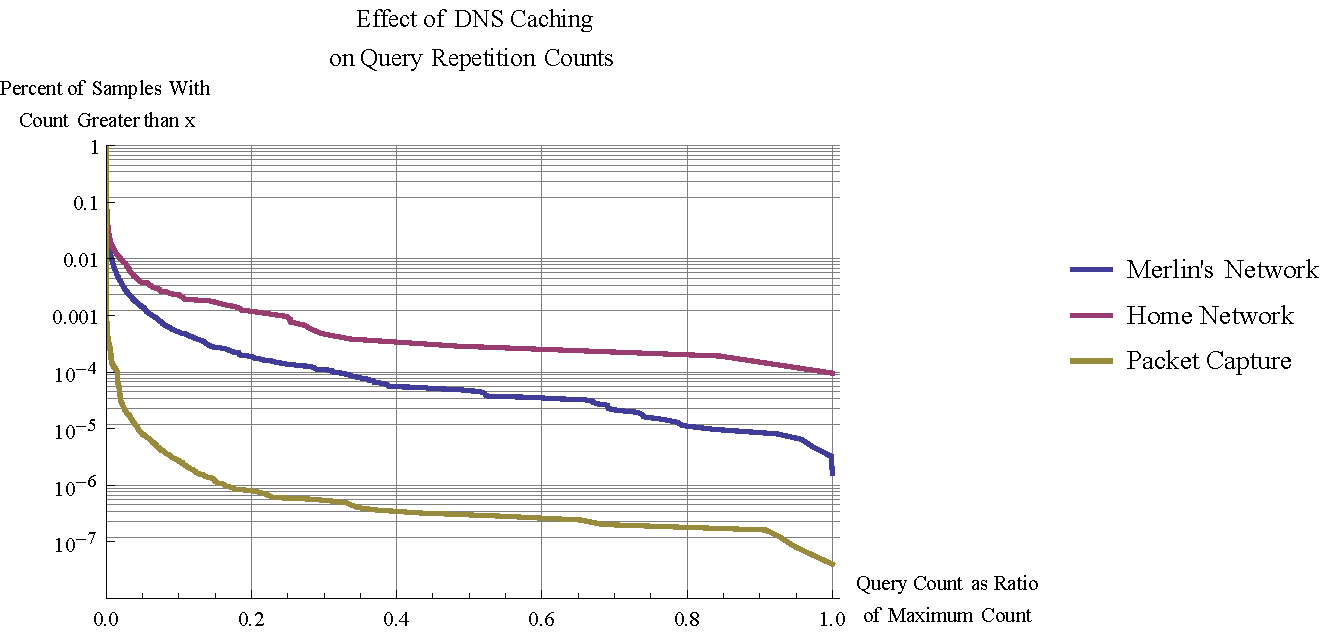
\includegraphics[width=0.75\textwidth]{../figures/caching.pdf}
\caption[Effect of DNS Caching on Query Counts]{Shows the trends for DNS query
counts in networks with and without caching. The axes are normalized to account
for the fact that the real world data has much more data than the home network.
By normalizing the query counts, it is possible to perform a direct comparison.}
\label{caching}
\end{figure}

%As can be seen
From the plot
%, which is logarithmic in the vertical axis, 
it is evident that the queries in an uncached environment occur over two
orders of magnitude more frequently than in a cached environment. This increased
occurrence in an uncached environment would have a strongly visible impact on
the naive metric's ability accurately detect DNS tunnels.
%The additional
%increase in the home network over the query logs from Merlin's network is due to
%the fact that there may be on-premise customer caching DNS servers on Merlin's
%network that are not, and can not be, accounted for in the logging obtained from
%Merlin.

As can be seen from the our method's underlying mechanisms, the DNS
caching actually provides a \emph{more pessimistic} detection
environment compared to the uncached environment. Unlike the naive
method, whose detection performance results will not be applicable in
an uncached environment, our method can be expected to
perform better in an uncached environment than in the testing in
Sect. \ref{detection-perf}.

%Born's method will also improve in detection performance in an uncached network,
%since it will cause normal traffic to have a character distribution more heavily
%skewed away from uniform, resulting in larger metrics and better certainty.
%Paxson's metric, however, will suffer in an uncached environment due to the fact
%that additional data, even if it is highly repetitive, will still increase the
%metrics of normal traffic and may obscure some low throughput DNS tunnels in the 
%process.

%\section{Implementation}
%\label{implementation}
%\subsection{General}
%
%The implementation specifics of this approach differ slightly between the C++
%and Python versions. The differences come primarily in efficiency and
%performance of the approach, with the C++ implementaiton designed for very high
%throughput applications. Both implementations, however, share a common
%architecture:
%
%\begin{itemize}
%
%\item The input is DNS queries and a timestamp at which the query was seen.
%
%\item The DNS query is broken down into a top-level domain (TLD) - such as
%\emph{google.com}, \emph{yahoo.ca} or similar - and the rest of the query - such
%as \emph{www} in \emph{www.google.com} and \emph{plus} in
%\emph{plus.google.com}.
%
%\item For each TLD, a data structure is created that maps queries to an integer,
%which represents the number of times that query was seen in the current
%interval.
%
%\item At the end of each time interval, the DLWE of each TLD is calculated, and
%the collection of TLD+DLWE pairs is output.
%
%\end{itemize}

%\subsection{C++}
%\label{cpp-implementation}
%The C++ implementation ingests raw packet data in the PCAP file
%format, relying on a purpose designed network protocol dissector for the
%extraction of the DNS query string, TLD, and any response information. The query
%timestamps are obtained from the packet header which is part of the PCAP format.
%
%The data structure used for storing the query-count mappings for each TLD is a
%custom high-performance, low memory usage, red-black tree written as part of
%libodb\cite{Friesen2013}. Computation of the DLWE for each TLD at the end of
%each interval is handled asynchronously in a separate thread so as not to block
%the ingestion of packets on the main thread. This asynchronous behaviour allows
%the processing to operate on very busy networks and allows for inherent and
%elegant non-blocking buffering of bursts of traffic beyond the processing rate
%of the host. This implementation is capable of processing in excess of four hundred
%thousand packets per second on commodity quad-core CPUs from 2011. The source
%code is included in the libodb source code distribution\cite{Friesen2013}.

\section{Detailed Testing Methodology and Processing Performance}
A collection of tests were run on several detection methods, demonstrating the
performance of our method when compared to existing methods
from the literature. The detection methods chosen for comparison are

\label{chosen-methods}
\begin{itemize}

\item The $n$-gram detection proposed by Born\cite{Born2010.cfa} because it is
well defined and was the most prevalent approach found during the literature
search. Additionally, the approaches built on this technique claim reasonable
success in detecting DNS tunnels.

\item The use of \emph{gzip} on domain and subdomain packet data as proposed by
Paxson\cite{Paxson2011} because it involves looking at data that is very similar
to the proposed approach, but makes use of
different methods for measuring the data throughput.

\item A naive approach that simply measures the volume (in number of characters
in the query strings) of packets per domain/subdomain in an attempt to
illustrate that simple volume of queries is a highly inadequate approach, and
that more sophisticated approaches can perform considerably better.
\end{itemize}

The collection of methods was put through several tests in an attempt to
demonstrate their performance in average (using existing implementations) and
worst case scenarios. All of the tests involving traffic generation were
performed in a virtual environment of two Linux-based virtual guests directly
connected via a virtual network on a single physical host. The tunnelling
applications were communicating between the virtual hosts, transmitting content
from the high entropy source \texttt{/dev/urandom} under Linux.

\subsection{Situational Performance Goals}
\subsubsection{Determining a Baseline}
\label{baseline}
Through cooperation with Merlin, an educational Internet Service Provider (ISP)
in Manitoba, DNS traffic was collected over a period from Thursday November 4
2010 until Friday November 26 2010. The hosts responsible for the DNS traffic
observed include several dozen school divisions totalling tens of thousands of
individual computers. The capture includes just over one billion packets
destined to, or sourced form, UDP port 53 (the standard DNS port).

This captured traffic will be used to determine a baseline distribution to which
the metrics produced on isolated tunnel traffic can be compared. This baseline
will provide context in order to determine if a method is able to detect a
tunnel with sufficiently high certainty.

It is assumed that the incidence of tunnels in this baseline traffic is
sufficiently low that it can be discounted. This assumption may not be perfectly
accurate due to to reasons indicated in the introduction.
%Because some security
%vendors use DNS to transmit some of their information, these transmissions are
%in essence a DNS tunnel and so will represent a certain portion of the real
%world traffic.
The effect of tunnels present in the real world traffic given the
assumption that there are none will result in a more pessimistic environment for
testing, since
%. Since some of the traffic that lies further out than the synthesized
%traffic may in fact be a tunnel, 
a portion of the false positive rate that the
detection approaches will suffer may actually be due to the classification of
existing traffic as a tunnel, and not due to misclassification.
%By making the
%assumption that no tunnels exist in the real world, however, the false-positive
%rates given here represent an lower bound and so should transfer well to other
%real-world scenarios.

\subsubsection{Existing Implementation Detection}
\label{test-existing}
This test will involve the two hosts communicating at varying throughput rates
using the chosen existing DNS tunnel implementations. The throughput rates will scale
from as little as several bytes per second, to as high as
the tunnel applications can support. The wide range of throughputs
used is done to give an indication of how the detection methods scale with
tunnelled throughput.

The existing implementations chosen for testing in this section are
Iodine\cite{iodinesrc}, DNScat\cite{dnscatsrc}, and DNS2TCP\cite{dns2tcpsrc}.
Iodine is chosen due to the fact that it provides a full VPN solution without
additional work by the user. DNScat is chosen due to being written in Java and
so runs on multiple platforms
%\footnote{DNScat will run on any platform that
%supports Java 1.4 or later\cite{dnscatsrc}}
 without the need for a compiler or
other complex dependencies that the user must obtain. DNS2TCP is chosen since it
does not require root access, and is written in C indicating potentially better
throughput than other mechanisms.

%The detection results of each of the approaches on the existing tunnelling
%applications is of value to those wishing to identify uses of DNS tunnelling
%currently in the wild. 
Instead of generating a large number of distinct events
that will be detected (or not) resulting in a ROC plot, rather a much smaller
number of prototypical events were produced.
%Details are given in Sect.
%\ref{chap-evaluation} regarding the statistics of the metrics from these tests
%and how the detection methods will be evaluated.
In essence, detection methods
will be scored for false-positive rate and ranked against each other in order to
determine a relative rating and ranking. The relative performance comparisons
allow for a more contextual performance analysis to be done between two methods
that perform very similarly.

%\section{Analysis Method Implementations}
%\label{implementations}
%\subsection{Common Scaffolding}
%\label{scaffolding}
%All implementations of the analysis methods are built on the same basic
%framework written in Python. The framework has the following basic properties:
%
%\begin{itemize} \item Unlike the C++ implementation of the proposed approach
%described in Sect. \ref{cpp-implementation}, which ingests raw PCAP formatted
%data, the Python scaffolding is unable to do so. Instead, the Python scaffolding
%relies on another tool to process raw packet captures (or other data sources
%such as DNS server logs) into a comma-separated value (CSV) file with a
%timestamp and a query string on each line.
%
%\item The scaffolding takes in two arguments: a file name to read the
%timestamp/query pairs from, and how long the intervals should be, in seconds.
%
%\item At the start of each interval, the main loop initializes an array to hold
%all of the queries for the upcoming interval. For the duration of the interval,
%the queries are added to the end of the array, which is passed to the analysis
%routine (where the specific detection method details are) at the end of the
%interval.
%
%\item When the queries from the interval are handed off for processing, each
%query has its top-level domain (TLD) identified, and then the rest of the query
%is passed to the specific method. The returned value is then assigned to the TLD
%that the query came from. At the end of each interval after processing each TLD,
%the digested values are output to the console.
%
%\item Once processing of the interval is complete and the information has been
%printed, the array is cleared in preparation for the beginning of the next
%interval.
%
%\end{itemize}

%There are some very important differences between the C++ implementation and
%this Python scaffolding that will cause the performance metrics to not be
%directly comparable.
%
%Unlike the C++ implementation which is designed for maximum performance and
%non-blocking ingestion of traffic, the Python implementations are poorly behaved
%around the ends of intervals where ingestion stops while processing occurs.
%Additionally, there is a reliance on another tool to produce the appropriate 
%input data. This removes the complexity of
%parsing and verifying the packet protocols from the performance figures for
%these implementations.
%
%\subsection{Naive}
%\label{implementation-naive}
%The metric returned for each query (stripped of its TLD) is simply the number of
%characters in the query. For each TLD, after all of the packets are processed,
%the total of all of the metrics for each query are summed together resulting in
%a single value that counts all of the characters that appeared in queries to
%that TLD.
%
%\subsection{Born}
%%Since the technique proposed by Born relies on having a notion of normal
%%traffic, a PDF of the character frequencies from the Alexa top one-million
%%domains was built (as is given in tables \ref{TABLE_dnssampling}) as the
%%baseline of normal. Additionally, this PDF was sorted from most to least
%%frequent character since the method relies on the assumption that DNS queries
%%approximately follow Zipf's Law, and not that they match the exact character
%%frequencies.
%
%Since Born's\cite{Born2010.cfa} assumption is that normal DNS queries
%approximately follow Zipf's Law, and that tunnels produce character
%distributions that are much closer to uniform, this was used to determine a
%metric. At the end of each interval, for each TLD all of the queries to that TLD
%are taken together and joined into a single long string. The character
%distribution of that string is then computed, and its standard deviation
%calculated.
%
%Since it is expected that tunnel traffic is close to uniform in its character
%distribution, it is then assumed that tunnels will have a very low standard
%deviation that continues to decrease as throughput (and thus amount of data per
%interval) increases while normal queries will have a standard deviation that
%increases very quickly by comparison.
%
%Because the next-gen tunnel
%used in the tests is designed to circumvent Born's detection method (and any
%other method that relies on character frequency analysis), it is expected that
%this approach will have poor detection performance on the next-gen tunnel.
%
%\subsection{Paxson}
%Paxson's\cite{Paxson2011} approach uses the \emph{gzip} utility to compress the
%queries to domains under the assumption that it will approximately measure the
%amount of unique data contained in those queries. Because \emph{gzip} is a
%command line interface to the underlying \emph{zlib} library, in Python this
%approach was implemented by making calls to Python's \emph{zlib} library and its
%\texttt{zlib.compress()} method.
%
%As with the previous implementations, the queries for each TLD over an interval
%are accumulated and joined together into a single long string. This string is
%then passed to the \texttt{zlib.compress()} method resulting in a compressed
%string whose length becomes the metric for that TLD in the current interval.
%
%Because Paxson's approach uses very similar assumptions, that DNS tunnels can be
%detected by measuring the amount of unique data transferred to each domain
%and/or subdomain, it is expected that Paxon's approach and the proposed approach
%will have very similar detection performance. However, due to the fact that
%Paxson's approach relies on a general-purpose compression library whereas the
%proposed approach uses a tailored algorithm and optimized data structures, it is
%expected that the proposed approach will have superior processing performance.
%
%\subsection{Proposed Approach}
%\label{proposed-method-python}
%In place of the high-performance red-black tree used in the C++ implementation,
%a Python \texttt{dict} was used in the Python implementation. The \texttt{dict}
%is used as a mapping from query strings (with the TLD removed) to integers
%indicating how many times that string appeared in the interval. At the end of
%each interval, such a mapping is built for every TLD from the packets seen in
%the interval, and for each TLD, the DLWE is computed from the obtained
%distribution. The computed DLWE is then used as the metric for the TLD for that
%interval.

\subsection{Tunneling Application Throughput}
\label{tunapptp}
The tunnelling applications used during the evaluation were subjected to
different rates of traffic in both client-to-server and server-to-client
directions. For each tunnelling application, sixteen captures were performed at
each of the following target throughput rates (in bytes per second) in each
direction (client-to-server and server-to-client where applicable):

10, 25, 50, 100, 250, 500, 1000, 2500, 5000, 10000, 25000, 50000, 100000,
250000, 500000, 1000000

The rates stop at ten bytes per second for practical reasons. It is considered
reasonable to assume that tunnels with a throughput rate lower than this are
ineffective at transmitting sufficient data to be practically useful in many
situations. As will be seen in Sect. \ref{chap-evaluation}, throughput rates
lower than ten bytes per second would quickly become lost in normal DNS
traffic for even the most discerning detection methods.

Due to implementation details of the applications, and of the next-gen tunnel,
not all applications were able to transmit traffic at the target rate. Figure
\ref{tunrates} shows how the various tunnelling applications responded to
various input rates, plotting their actual rate of ingestion of input and the
observed number of characters of query output they generated on the network.
%Note that for the lighter coloured graphs showing the observed output, the
%vertical axis is representing a value equivalent to the naive metric. 
The
next-gen tunnel was not tested in a server-to-client direction since it does not
implement that functionality.

\begin{figure}[h]
\centering
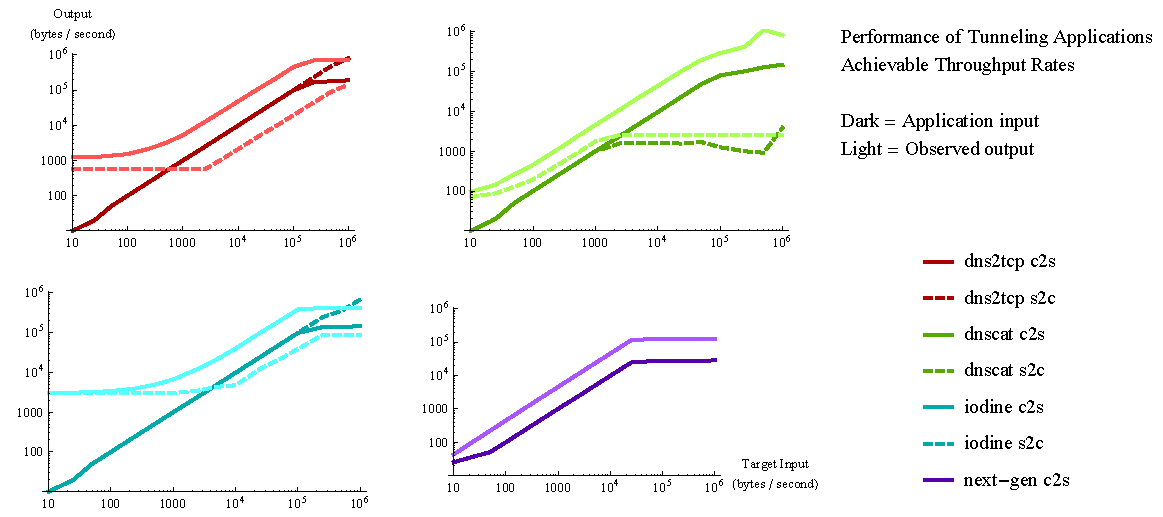
\includegraphics[width=\textwidth]{../figures/tunrates.pdf}
\caption[DNS Tunneling Application Throughput Scaling]{Shows the scaling
behaviour of DNS tunnelling applications as the input rate is scaled up. Note
that not all applications are capable of transmitting data at the rate they are
given data, which is visible as a plateau on the right-hand-side of each plot.}
\label{tunrates}
\end{figure}

\subsection{Detection Method and Python Interpreter Processing Performance}
\label{processing-perf}
Python has several interpreters available freely in addition to the standard
interpreter (for this discussion, the standard interpreter will be referred to
as Cython). A notable alternative, called PyPy, is a Python interpreter written
in Python itself that contains just-in-time compilation (JIT) mechanisms that
Cython does not have. PyPy can offer an order of magnitude
or better speedup\cite{pypyvc-strfmt} in some workloads. Figures \ref{pmat}, \ref{pmqr}, and \ref{pmqr-100k} show
the performance of the various detection methods over aggregate tunnel and
real-world data on both PyPy and Cython.

%Figure \ref{pmat} shows that, on tunnel data, the analysis methods under Cython
%all suffer, to varying degrees, as the amount of data to process per interval
%increases. The naive and proposed methods suffer the least, while Paxson's
%method suffers by far the most, dropping to approximately half of its original
%processing rate. Note that Born's method and Paxson's method trade places as the
%slowest performer at a throughput of approximately five kilobytes of data per
%second.
%
%When looking at PyPy performance, with the exception of a dip around one
%kilobyte of data per second, performance increases as the amount of data
%increases in direct contrast to the behaviour of Cython. This increase in
%performance can be due to the JIT components having enough time to achieve some
%measurable optimizations of common code-paths. In addition, the general ranking
%of the algorithms by performance is maintained (with the exception of the swap
%of Born and Paxson seen under Cython) from Cython to PyPy. Despite this
%improvement, the average performance is still nearly an order of magnitude below
%that of Cython in many of the cases.

\begin{figure}[h]
\centering
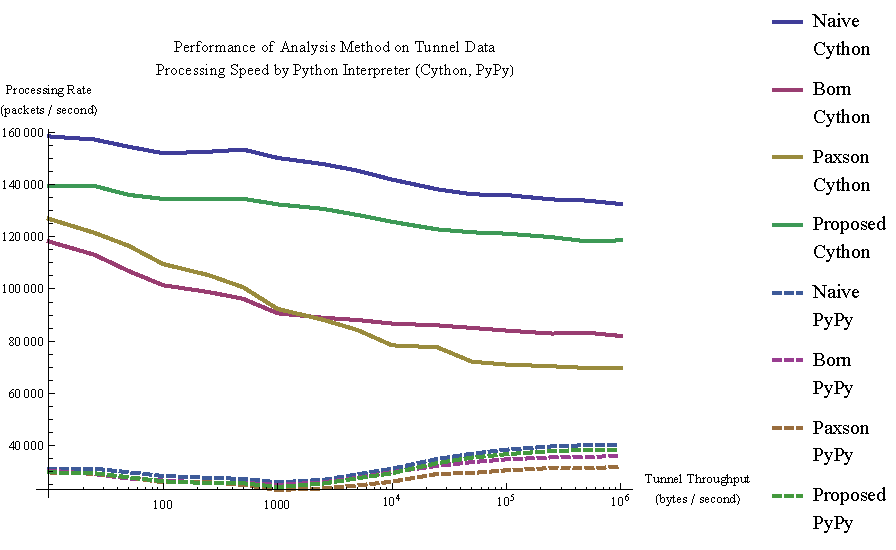
\includegraphics[width=0.75\textwidth]{../figures/pmat.pdf}
\caption[Performance of Analysis Method and Python Interpreter on Aggregate
Tunnel Data]{This plot shows the performance of the detection methods and Python
interpreters over the aggregate tunnel data. The output is packet processing
rate as a function of the target input rate (rate at which the tunnels are
transmitting traffic). 
%As the target input rate increases, the structures
%involved in the methods get larger in a non-linear way, resulting in longer
%operation times and slower performance.
}
\label{pmat}
\end{figure}

%Figure \ref{pmqr} shows the performance over time of the different detection
%methods and Python interpreters as more packets are ingested from real world
%data. Observe that as time progresses, the methods get progressively slower,
%likely due to inefficiencies in the interpreter and/or method.

%Also unlike the aggregate tunnel detection performance, the methods when run
%under PyPy perform \emph{far} better, even surpassing the Cython counterparts in
%at least one case. Note that the Paxson's approach when run under PyPy shows
%decreasing performance over time while no such decrease for larger times is
%observed when run under Cython.

%%\begin{figure}[h]
%%\centering
%%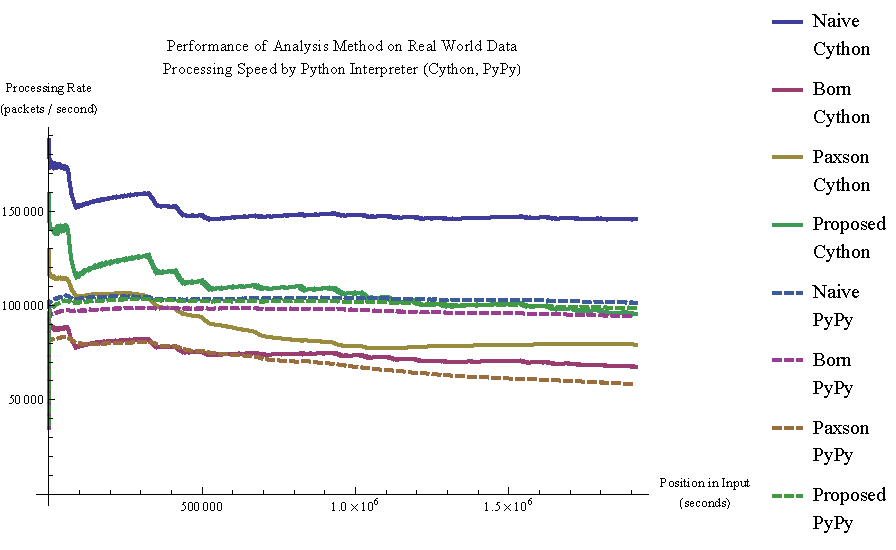
\includegraphics[width=0.75\textwidth]{../figures/pmqr.pdf}
%%\caption[Performance of Analysis Method and Python Interpreter on Real World
%%Data]{This plot shows the performance of the detection methods and Python
%%interpreters on real world DNS traffic. The output is packet processing performance as time
%%progresses and more packets are processed by the script. As more packets are fed
%%into the script, inefficiencies in the methods and/or the Python interpreters
%%themselves become observable in the degradation of performance.}
%%\label{pmqr}
%%\end{figure}

\begin{figure}[h]
\centering
\subfigure[Full data set]{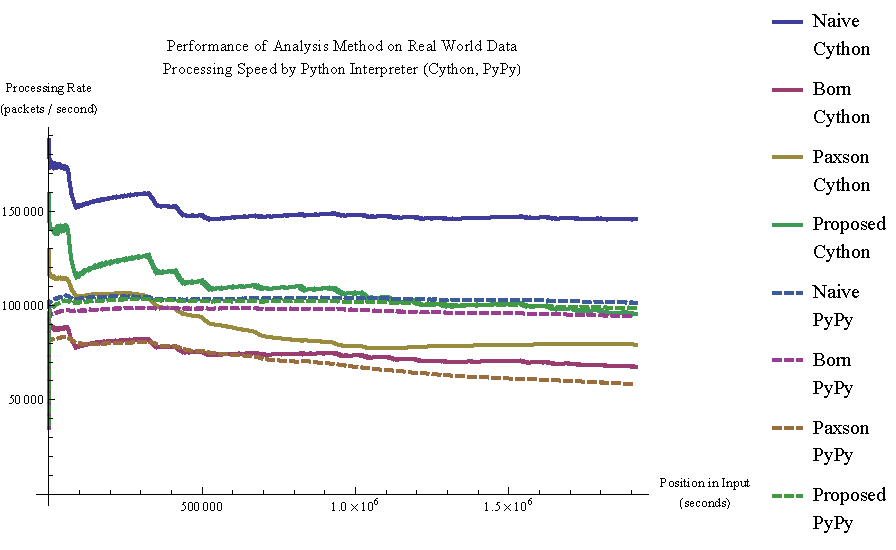
\includegraphics[width=0.48\textwidth]{../figures/pmqr.pdf}\label{pmqr}}
\subfigure[Early time]{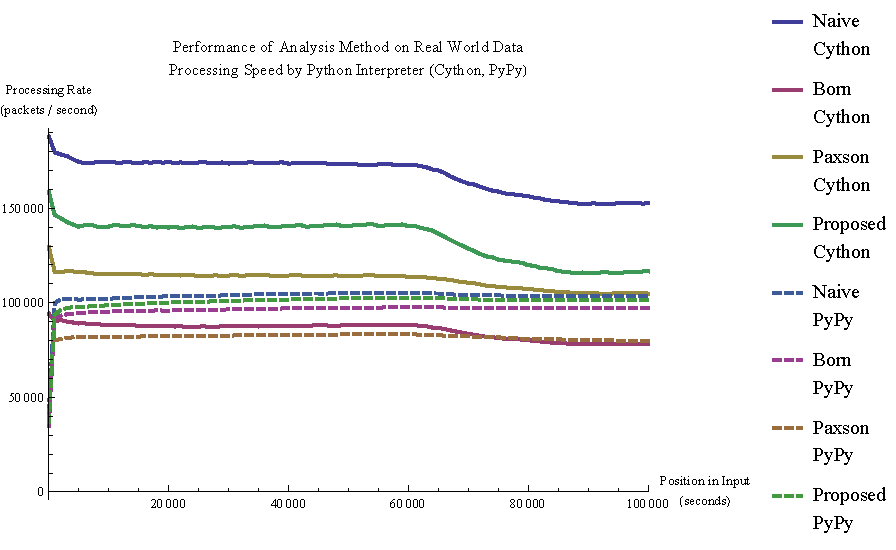
\includegraphics[width=0.48\textwidth]{../figures/pmqr-100k.pdf}\label{pmqr-100k}}
\caption{Performance of Analysis Method and Python Interpreter on Real World Data}
\end{figure}

Figure \ref{pmqr} shows the performance of the detection methods and Python
interpreters on real world DNS traffic. The output is packet processing performance as time
progresses and more packets are processed by the script.
%As more packets are fed
%into the script, inefficiencies in the methods and/or the Python interpreters
%themselves become observable in the degradation of performance.

%Figure \ref{pmqr-100k} shows the same data, but with a limited scale allowing
%early-time behaviour to be examined. Note that the ramp-up of PyPy's JIT
%components is observed in the very early time followed by a very consistent
%processing rate.

%%\begin{figure}[h]
%%\centering
%%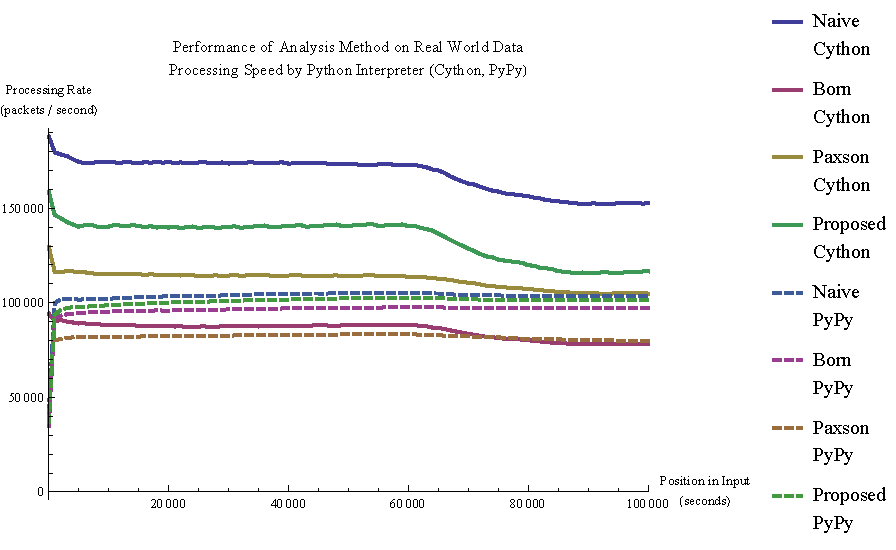
\includegraphics[width=0.75\textwidth]{../figures/pmqr-100k.pdf}
%%\caption[Performance of Analysis Method and Python Interpreter on Real World
%%Data - Early Time]{This plot is identical to Fig. \ref{pmqr} but restricts the time
%%displayed to the first one hundred thousand seconds. The 'spool up' of the JIT
%%portion of PyPy is noticeable in the very early time-scales.}
%%\label{pmqr-100k}
%%\end{figure}

Figure \ref{pmqr-100k} is identical to Fig. \ref{pmqr} but restricts the time
displayed to the first one hundred thousand seconds. The 'spool up' of the JIT
portion of PyPy is noticeable in the very early time-scales.

%Figures \ref{ppia-born}, \ref{ppia-naive}, \ref{ppia-paxson}, and \ref{ppia-proposed} attempt 

Figure \ref{ppia-all} attempts
to represent the performance of the various
detection methods and Python interpreters as more tunnel data is moved through
them per interval. Their horizontal axes are the actual data input rate (see \ref{tunapptp}), and the vertical axes indicate the
processing rate (in packets per second).

In Fig. \ref{ppia-all} the legend requires some additional context. The
plot legends contain labels of the form \emph{dns2tcp c2s Cython} which contains
three distinct pieces of information. The first word indicates which tunnelling
application being one of DNS2TCP, DNSCat, Iodine, or the next-generation simulated application which is indicated by a name of \texttt{next-gen}. The
second word indicates whether the data being moved over the tunnel is being
transferred from the client to the server (\texttt{c2s}) or from the server to
the client (\texttt{s2c}). The final word indicates which Python interpreter is
being used.

There are fourteen lines on each figure, each corresponding to a Python
interpreter, tunnel application, and data transfer direction triple. The solid
lines correspond to runs made under the Cython interpreter and dashed lines
indicate the use of the PyPy interpreter.

\begin{figure}[h]
\centering
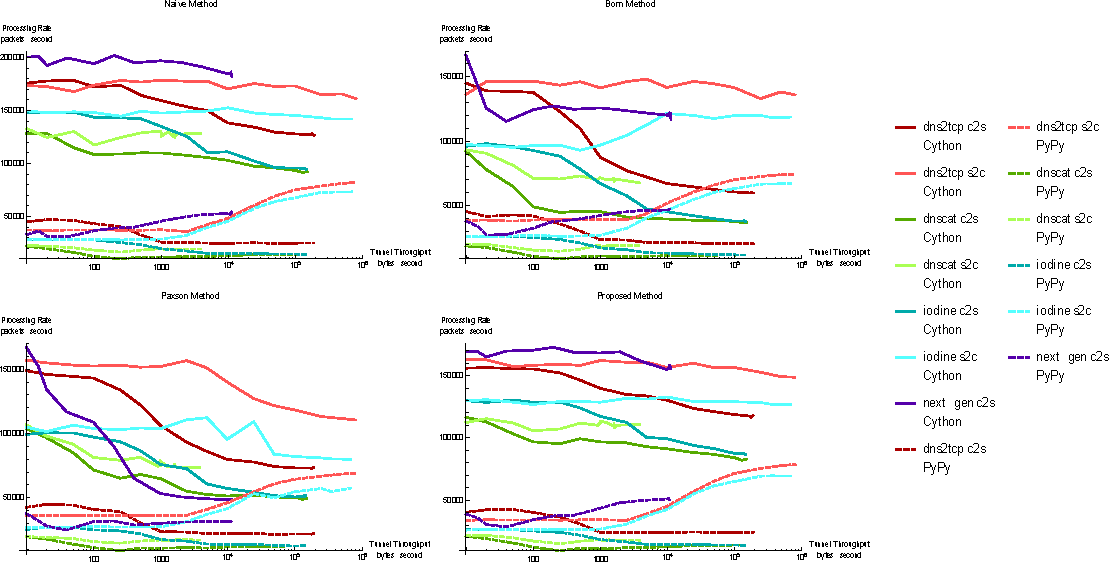
\includegraphics[width=\textwidth]{../figures/ppia-all.pdf}
\caption[Performance of Alls Method on Tunnel Data by Python
Interpreter]{Performance of all methods on separated tunnelling application
data, showing processing rate as a function of input rate.}
\label{ppia-all}
\end{figure}
%%
%%\begin{figure}[h]
%%\centering
%%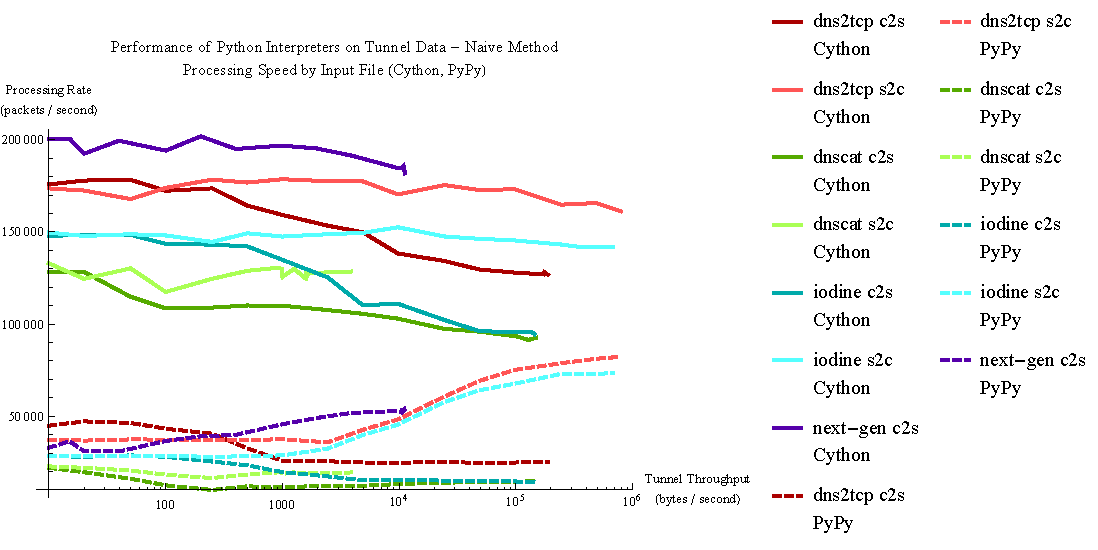
\includegraphics[width=0.75\textwidth]{../figures/ppia-naive.pdf}
%%\caption[Performance of Naive Method on Tunnel Data by Python
%%Interpreter]{Performance of the naive method on separated tunnelling application
%%data, showing processing rate as a function of input rate.}
%%\label{ppia-naive}
%%\end{figure}

%The performance of the naive method has very little dependence on the input
%rate, suffering minimally as the amount of data per interval increases. This is
%expected behaviour since Python's string objects allow for efficient computation of
%length, being of $O(1)$ computational complexity\cite{python-strlencplx}.
%Because the naive method's implementation must calculate the length of each
%query, additional queries increase the time complexity of the method linearly
%with the number of queries that must be processed. The Iodine and DNS2TCP
%client-to-server transfers show marked drops in performance, potentially due to
%longer queries being used which would increase the time taken to read the files
%into the script.
%
%The PyPy performance figures show similar clustering to the Cython plots, with
%the notable exception that the DNS2TCP and Iodine server-to-client performance
%improves drastically for higher throughputs. This is again likely due to the JIT
%components of PyPy being able to optimize for runtime conditions. Despite this
%improvement, they still perform at approximately half the rate of their Cython
%counterparts at the most favourable throughputs.

%%\begin{figure}[h]
%%\centering
%%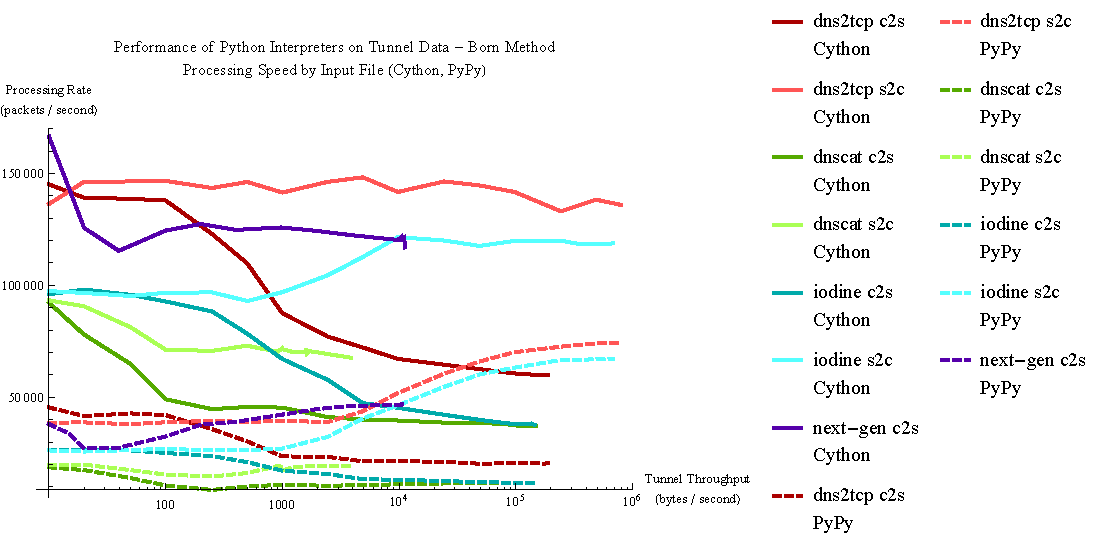
\includegraphics[width=\textwidth]{../figures/ppia-born.pdf}
%%\caption[Performance of Born's Method on Tunnel Data by Python
%%Interpreter]{Performance of Born's method on separated tunnelling application
%%data, showing processing rate as a function of input rate.}
%%\label{ppia-born}
%%\end{figure}

%Born's approach shows a very high level of variation in performance, with marked
%decreases in processing rate as the throughput is increased for many of the the
%tunnel applications. Notable exceptions are the Iodine and DNS2TCP
%server-to-client transfers which suffer minimal degradation or improve as
%throughput increases respectively. Again, the same patterns as with the naive
%approach are seen under the PyPy runs, however relative performance overall is much
%better from PyPy. This is in part due to the much larger performance hit taken
%by the Cython implementations. This performance is likely due to the fact that
%the Python implementation of Born's approach makes use of a collection of loops
%and arithmetic. This type of computation is not well optimized under Cython but
%can be subject to excellent run-time optimization under PyPy's JIT components.
%PyPy is still, however, unable to improve upon, or match, Cython's performance in these
%workloads.

%%\begin{figure}[h]
%%\centering
%%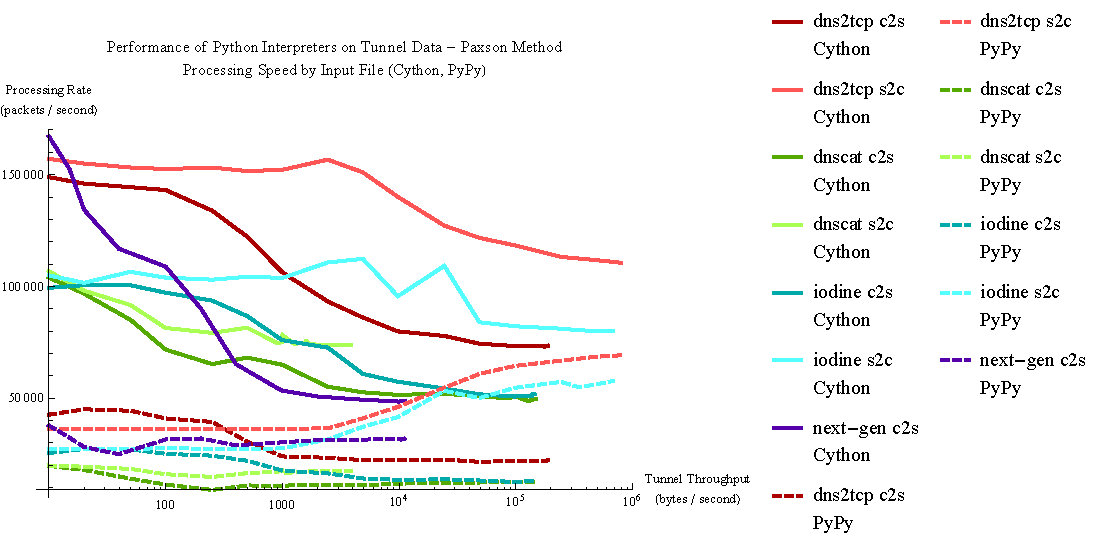
\includegraphics[width=\textwidth]{../figures/ppia-paxson.pdf}
%%\caption[Performance of Paxson's Method on Tunnel Data by Python
%%Interpreter]{Performance of Paxson's method on separated tunnelling application
%%data, showing processing rate as a function of input rate.}
%%\label{ppia-paxson}
%%\end{figure}

%Very similar behviour is again seen in the performance of Paxson's approach as
%compared to Born's, with Cython out-performing PyPy and a general
%trend of performance degradation with additional throughput.

%%\begin{figure}[h]
%%\centering
%%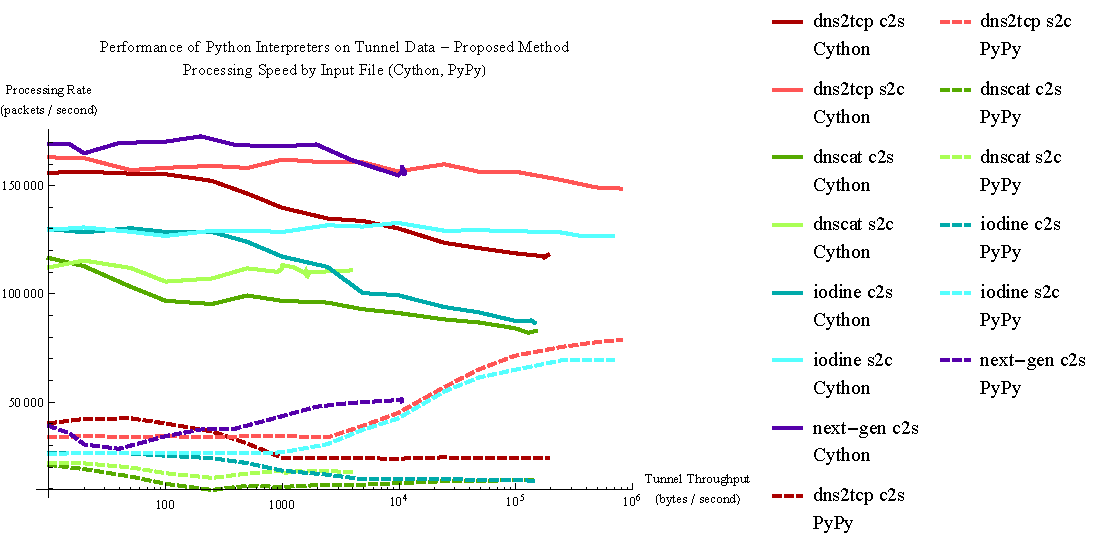
\includegraphics[width=\textwidth]{../figures/ppia-proposed.pdf}
%%\caption[Performance of the Proposed Method on Tunnel Data by Python
%%Interpreter]{Performance of the proposed method on separated tunnelling
%%application data, showing processing rate as a function of input rate.}
%%\label{ppia-proposed}
%%\end{figure}

Our approach shows performance characteristics and trends that match
the naive approach far more closely than either of the other two approaches.
There is minimal degradation in performance for most of the tunnelling
applications, and almost all of the samples under the Cython interpreter are
above one hundred thousand packets per second.

It is instructive to observe that PyPy's performance overall is considerably
lower than Cython on tunnel data, but as is shown in Fig. \ref{pmqr}, this is
not the case on real-world data.

\subsection{Processing Performance Conclusion}
%As has been shown, the detection methods were tested on both real world and
%purpose-generated tunnel application traffic as well as on two different Python
%interpreters and were instrumented for their processing performance.

When evaluating the performance of the detection methods on real-world data, in all
cases the naive method is the fastest, followed by our approach, Born's
method, and Paxson's method in order.

When operating on tunnelling application traffic, the average performance of the
methods (averaged over all tunnels and cases) can be seen in Fig. \ref{pmat}
where the our method and the naive method both perform well, maintaining processing
rates in excess of one hundred twenty thousands packets per second. Born's and
Paxson's approaches both suffer severe degradation of performance as throughput
increases, resulting in final processing rates well below one hundred thousand
packets per second.

\begin{figure}[h] \centering
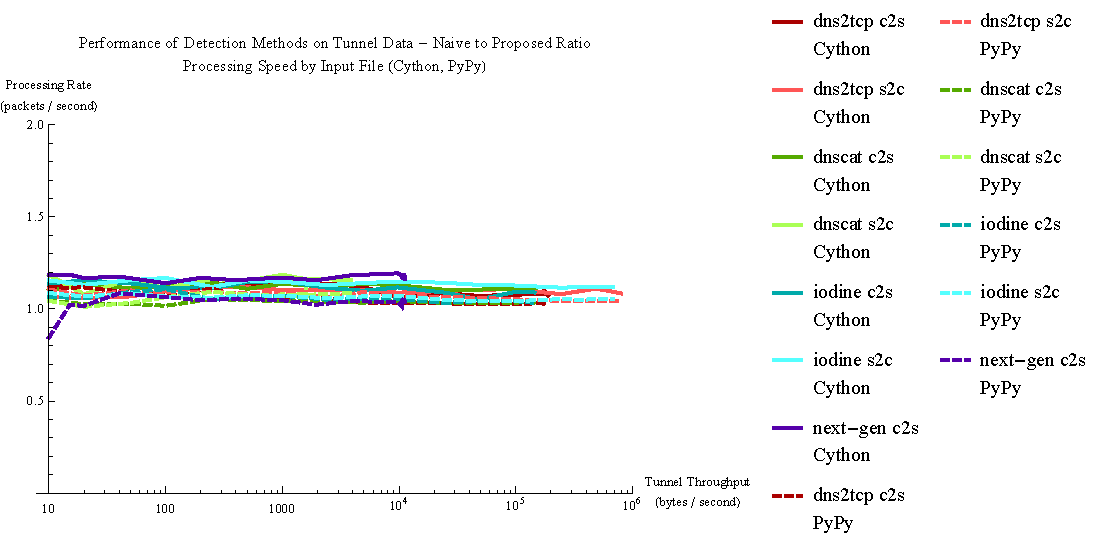
\includegraphics[width=0.75\textwidth]{../figures/ppia-naive2proposed.pdf}
\caption[Performance Ratio of the Naive Method to the our Method on Tunnel
Data by Python Interpreter]{The ratio of the performance of the naive method to
our method on separated tunnelling application data, with the vertical
axis showing the speedup of the naive method over our method.}
\label{ppia-naive2proposed} \end{figure}

When the ratio of the performance of the naive method to our method is
examined, a clustering very close to a fixed value is observed as in Fig.
\ref{ppia-naive2proposed}. This indicates that much of the performance
degradation, and potentially other performance characteristics, of the two
methods are dominated by the common scaffolding and/or the Python interpreter as
opposed to the underlying methods or their implementation.

Through this examination, it has been shown that our method
out-performs both methods from the literature by a considerable margin and comes
very close to matching the naive method in performance in many cases.

\section{Tunnel Detection Evaluation}
\label{chap-evaluation}
\label{tunnel-detection-performance}

In order to obtain the metrics used in this section, tunnel application and real
world data was separated into adjacent ten second windows for processing. The
distribution of metrics across these windows is computed and used to produce the
plots for real world data as well as indicative representative values for tunnel
applications.

When examining the distribution of metrics produced by tunnel applications, it
was discovered that the metrics were clustered extremely tightly around the
mean. The relative standard deviation for the various tunnel applications,
transfer directions (server-to-client or client-to-server) are given as a
function of input rate for each of the detection methods in
%plots \ref{rsd-naive}, \ref{rsd-born}, \ref{rsd-paxson}, and \ref{rsd-proposed}
Fig. \ref{rsd-all}
. These
plots show that the clustering around the mean for these metrics is so tight
that a standard receiver operating characteristic (ROC) plot would be of little
additional value since the true and false positive rates are dependant on the
value ranges that the metrics take. Since the range of values that the metrics
take on is so limited, the differences between a low and high percentile in true
and false positive rates would be minimal to statistically insignificant.

\begin{figure}[h]
\centering
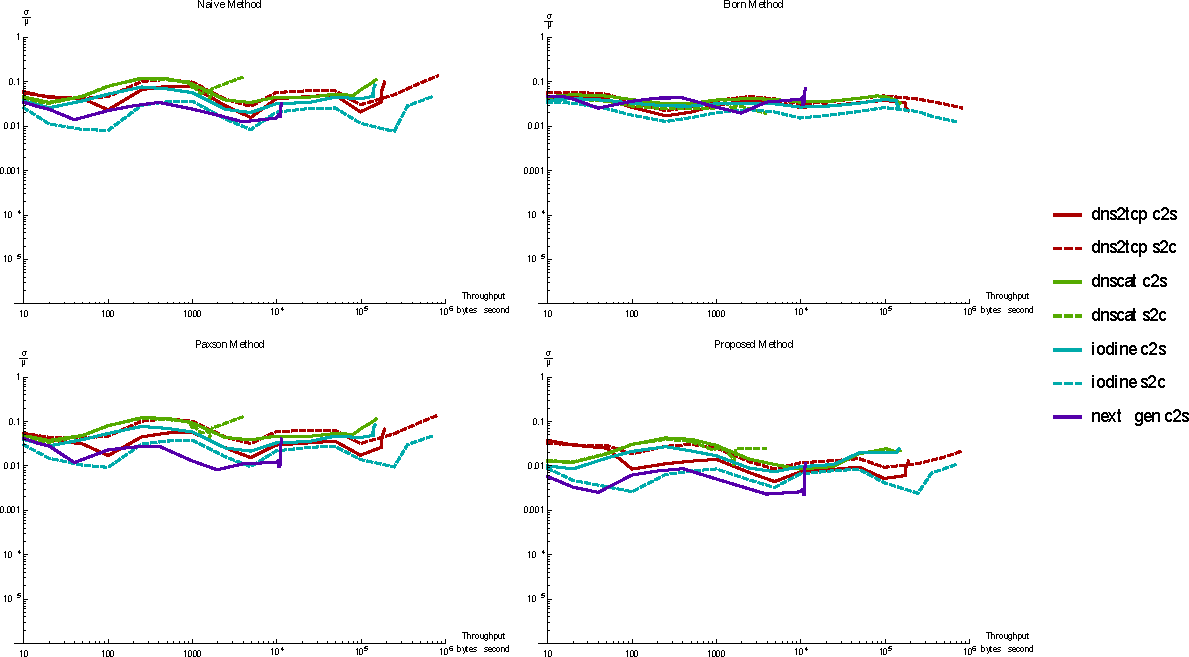
\includegraphics[width=\textwidth]{../figures/rsd-all.pdf}
\caption[Relative Standard Deviation of Metrics - All Metrics]{Relative Standard Deviation of Metrics - All Metrics}
\label{rsd-all}
\end{figure}

%\begin{figure}[h]
%\centering
%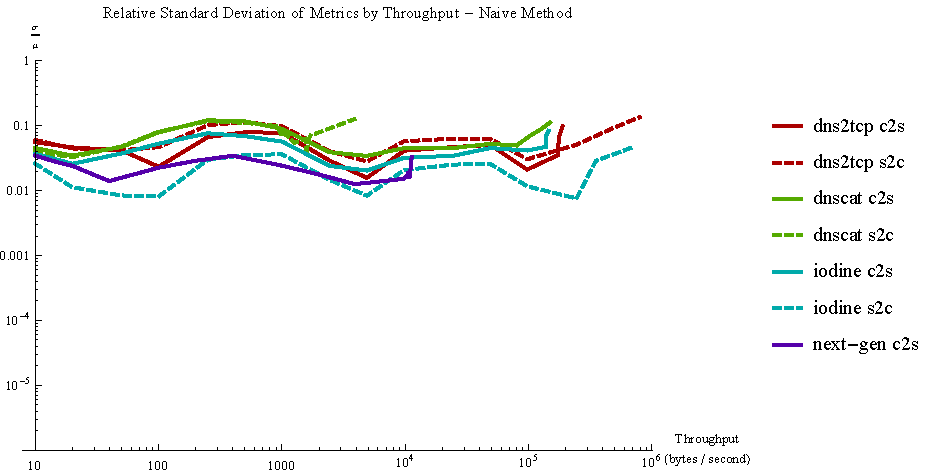
\includegraphics[width=\textwidth]{../figures/rsd-naive.pdf}
%\caption[Relative Standard Deviation of Metrics - Naive Metric]{Relative Standard Deviation of Metrics - Naive Metric}
%\label{rsd-naive}
%\end{figure}
%
%\begin{figure}[h]
%\centering
%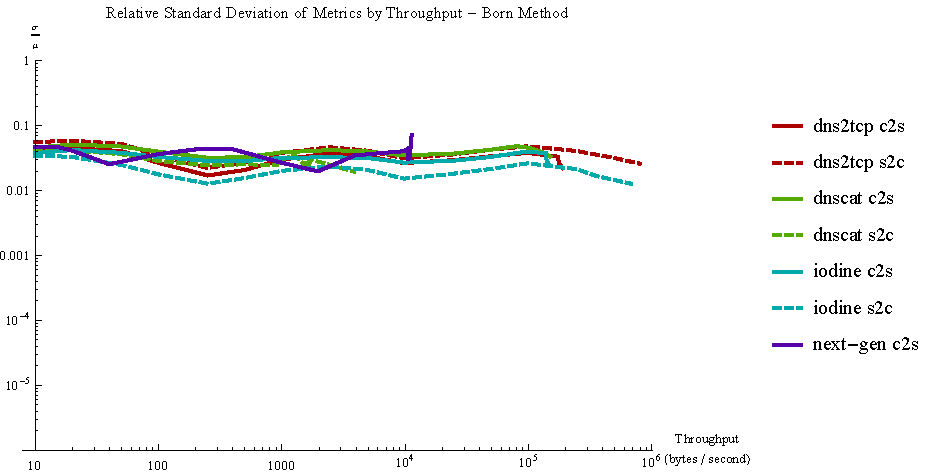
\includegraphics[width=\textwidth]{../figures/rsd-born.pdf}
%\caption[Relative Standard Deviation of Metrics - Born Metric]{Relative Standard Deviation of Metrics - Born Metric}
%\label{rsd-born}
%\end{figure}
%
%\begin{figure}[h]
%\centering
%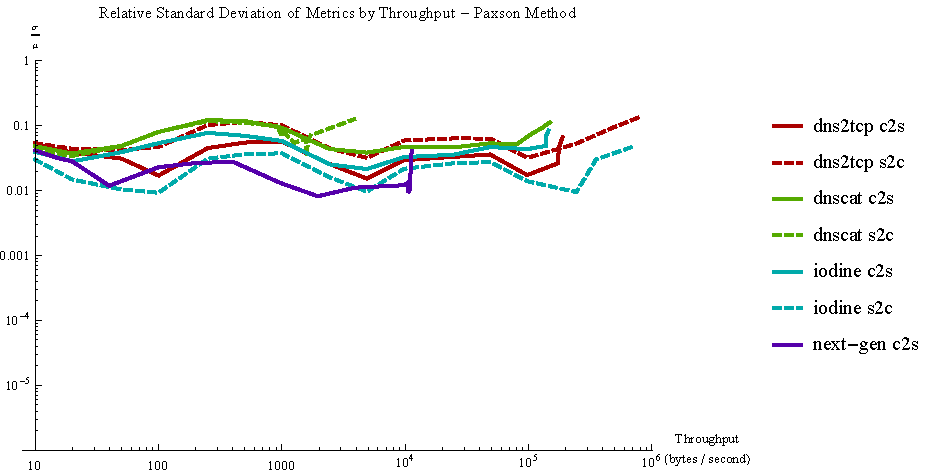
\includegraphics[width=\textwidth]{../figures/rsd-paxson.pdf}
%\caption[Relative Standard Deviation of Metrics - Paxson Metric]{Relative Standard Deviation of Metrics - Paxson Metric}
%\label{rsd-paxson}
%\end{figure}
%
%\begin{figure}[h]
%\centering
%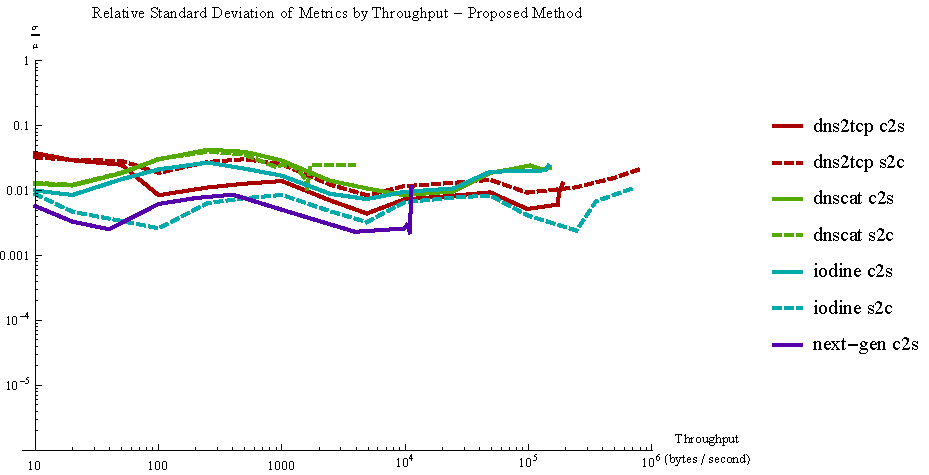
\includegraphics[width=\textwidth]{../figures/rsd-proposed.pdf}
%\caption[Relative Standard Deviation of Metrics - Proposed Metric]{Relative Standard Deviation of Metrics - Proposed Metric}
%\label{rsd-proposed}
%\end{figure}

Because of the extremely tight distributions and the insensitivity on input data
distribution (described in Sect. \ref{chosen-methods}), the mean value will be
taken as representative of the tunnel metric for a given throughput, direction,
detection method, and tunnel application. This choice of a single representative
value simplifies discussion and makes presentation of the salient
characteristics of the detection methods more straight forward.

Figure \ref{mbtt} shows several log-log plots (in order to be able to provide
adequate resolution for both very small and very large throughputs), one for
each detection method, that demonstrates how the mean metric generated by the
methods scale as the throughput of the tunnel is increased.
%The expected trends
%of the detection methods is as follows:

%\begin{itemize}
%\item The naive metric is expected to increase with throughput with a slope
%dependant on the implementation. In practice, all of the implementations have a
%slope of approximately one indicating that no significant inflation of the input
%data takes place (beyond that incurred by encoding to base 32 or 64 as the
%implementation may choose).
%
%\item Born's metric is expected to decrease to zero for tunnels as their
%character distribution approaches uniform. The character distribution of tunnel
%traffic is not directly tied to throughput, but rather has an implicit
%dependency on it due to the law of large numbers. Since the distribution is
%approximately uniform in the limit, there needs to be enough sample data before
%the distribution begins to converge and the effects of small-scale variations
%begin to average out.
%
%This is the behaviour seen for most tunnels with the exception of the Iodine and
%DNS2TCP server-to-client transfers as well as the next-gen tunnel. The next-gen
%tunnel's behaviour is precisely as expected due to its construction specifically
%to evade character frequency analysis such as is used in Born's approach.
%
%\item Paxson's metric is expected to increase approximately linearly with a
%slope that depends on the implementation and on the compressibility of the
%transferred data. Because the transferred data is pseudorandom, it is nearly
%incompressible and thus the observed slops of the lines is derived from the
%implementation details of the various tunnelling applications.
%
%\item The proposed metric is expected to increase approximately logarithmically
%with additional throughput due to its reliance on entropy as a multiplicative
%factor in its final metric. This is the behaviour seen for all except
%Iodine's server-to-client transfer, with varying scaling factors.
%
%\end{itemize}

%\begin{landscape}
\begin{figure}[h]
\centering
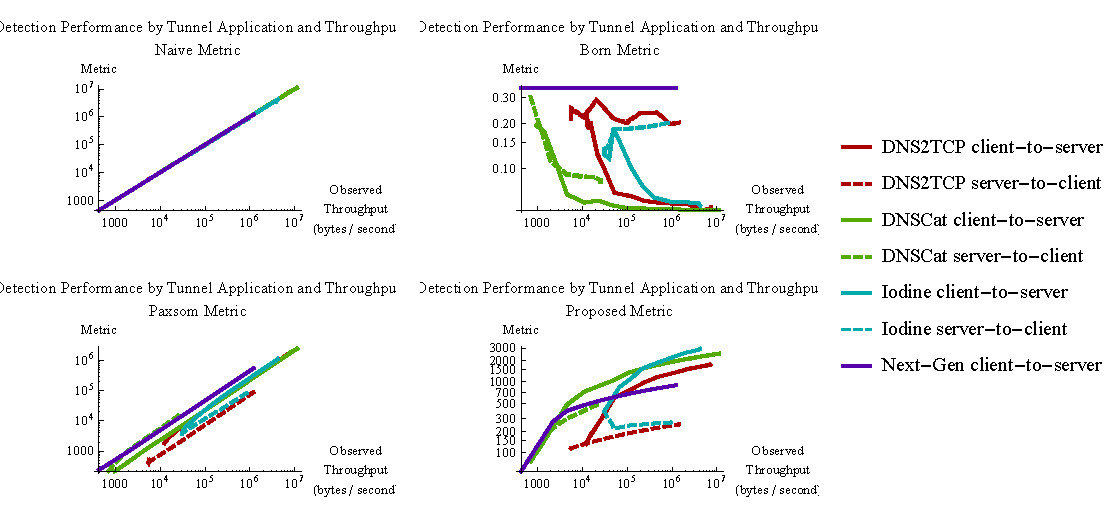
\includegraphics[width=\textwidth]{../figures/mpbtt.pdf}
\caption[Scaling of Detection Metrics by Tunnel Throughput]{These plots show how
the metrics computed by the various detection methods scale per tunnelling
application as a function of the tunnel throughput rates. Note that since not
all tunnels are capable of a full range of throughputs (some generate a minimum
amount of traffic, regardless of how low the throughput is), resulting in some
of the shorter plots.}
\label{mbtt}
\end{figure}
%\end{landscape}

As is visible in Fig. \ref{mbtt}, tunnels with lower throughput produce
categorically smaller (or in the case of Born's approach, larger) metrics. This
property of the lower throughput tunnels makes them necessarily harder to detect
when laid over top of normal traffic. Because of this, the methods will be
tested on their ability to detect the most hidden tunnel of each application,
which in practice is one of the tunnels that transmits only ten bytes per
second, against background normal DNS traffic. By testing
the methods to ensure they detect low-rate tunnels, their ability to detect
high-rate tunnels is implicitly demonstrated.

It is instructive to observe the relative standard deviations for the various
tunnel applications and detection methods at the lowest throughput level, ten
bytes per second. This is given in Table \ref{rsd-minimum}.

%This tight packing of samples indicates that the normal method of classifying
%detection methods, that is the \emph{receiver operating curve (ROC)}, may not be
%entirely appropriate. Since the data sets involved are not annotated in the
%sense that abnormal events to be detected are identified from normal traffic,
%the concept of a 'true positive' does not exist. Similarly, the concept of true
%and false negatives are equally inapplicable. This leaves false positives as the
%most reasonable metric. Further, since ROCs use the percentile of sample value
%as an axis of display, the tight packing of the samples would result in curves
%that do not convey as much information as in a less tightly packed situation.
%For these reasons, a single representative value in each case (the mean), is
%chosen to represent the collection of values, allowing more information per plot
%to provide context.

\begin{table}[ht]
\centering
\begin{tabular}{r|cccc}
& \,\,\,\,Naive\,\,\,\, & \,\,\,\,Born\,\,\,\, & \,\,Paxson\,\, & Proposed \\
\hline
%DNS2TCP c2s & 0.0559644 & 0.0497584 & 0.0450118 & 0.0371504 \\
%DNS2TCP s2c & 0.0477585 & 0.0675144 & 0.0495964 & 0.0392231 \\
%DNSCat c2s & 0.0155828 & 0.0526164 & 0.018919 & 0.00980975 \\
%DNSCat s2c & 0.0152077 & 0.0452746 & 0.0172972 & 0.0101241 \\
%Iodine c2s & 0.00720872 & 0.0439898 & 0.0106345 & 0.00500239 \\
%Iodine s2c & 0.00687431 & 0.0377363 & 0.0119256 & 0.00375623 \\
%Next-Gen & 0.0309484 & 0.0581522 & 0.0399604 & 0.00414985 \\
DNS2TCP c2s & 0.056 & 0.050 & 0.045 & 0.037 \\
DNS2TCP s2c & 0.048 & 0.068 & 0.050 & 0.039 \\
DNSCat c2s & 0.016 & 0.053 & 0.019 & 0.0098 \\
DNSCat s2c & 0.015 & 0.045 & 0.017 & 0.010 \\
Iodine c2s & 0.0072 & 0.044 & 0.011 & 0.0050 \\
Iodine s2c & 0.0069 & 0.038 & 0.012 & 0.0038 \\
Next-Gen & 0.031 & 0.058 & 0.040 & 0.0041 \\
\end{tabular}
\caption[Relative Standard Deviation of Lowest Throughput Tunnel by Detection Method and Tunnel Application]{The relative standard deviation given by $\frac{\sigma}{\mu}$ of the multiple samples for each tunnel application and detection method pairing for the lowest throughput rate.}
\label{rsd-minimum}
\end{table}

\subsection{Detection Performance Against Real World Data}
\label{detection-perf}

Since tunnel metrics are represented by a single value, the mean of their
samples for a given scenario, the detection methods will be ranked based on how
they partition the metrics produced by real world data. For simplicity a
thresholding approach will be considered as the classification mechanism, with
anything below the tunnel's metric classified as legitimate, and anything above
the tunnel's metric classified as a tunnel. Detection methods will be scored
based on the number of false positives that could be expected to occur given the
distribution obtained for normal traffic. The ordering is reversed for Born's method.

For each detection method, two plots are given that show how the tunnel
applications compare to real world data. The first plot demonstrates how the estimated
false-positive rate behaves as a function of throughput rate, direction, and
tunnel application. The second plot shows the distribution of metrics of real
world data with indicators represented by vertical coloured bars placed to mark
the mean metrics of various tunnel application and direction pairs as given in
the corresponding legend. For each marker, the false-positive rate is the $y$
value of the normal traffic curve at intersection of the normal curve with the
vertical marker. The second plot only shows the tunnelling combinations that
produce the highest false-positive rates, since those are the scenarios of
greatest interest. These eight plots are shown in Fig. \ref{mpn} to Fig. \ref{mph}.

%The plots shown here illustrate how the various tunnel application fare when
%compared to normal traffic. On each plot the vertical axis is "percent of
%samples with a metric greater than $x$" with the horizontal axis being the
%metric produced by the method. The black curve represents normal traffic, with
%the vertical coloured bars representing the various DNS tunnels. The vertical bars,
%coloured and dashed/solid according to the legend, mark the target throughput
%levels given in section \ref{tunapptp}, but are not identified otherwise. As can
%be seen in figure \ref{mbtt}, in almost all cases (with any exceptions occurring for higher throughputs), the metric is approximately
%monotonic with the lowest throughput samples having the smallest metric. Due to
%the plot ranges on the following figures, not all bars are visible on all plots.
%Due to the tendency of Born's metric to produce small values for tunnels, most
%of the tunnel bars are visible on the plot of Born's metric.
%
%Due to the layout of the plots, the approximate detectability of a tunnel is
%related to the $y$ value of the crossing of the vertical markers with the normal
%curve. This crossing indicates how near the outliers the marker sits with an
%intersection at $y$ values very near 0 or 1 representing the best detection
%probability. The closer to the outliers the tunnel is measured to be, the less
%ambiguity there is as to whether or not the analyzed traffic represents normal
%traffic or not. A value of 0 or 1 would indicate a perfectly detectable tunnel,
%while a value of 0.5 would indicate a tunnel that suffers from a very high
%ambiguity of classification. This value will be referred to as the
%\emph{crossing value} in subsequent discussion.

%%%\begin{figure}[h]
%%%\centering
%%%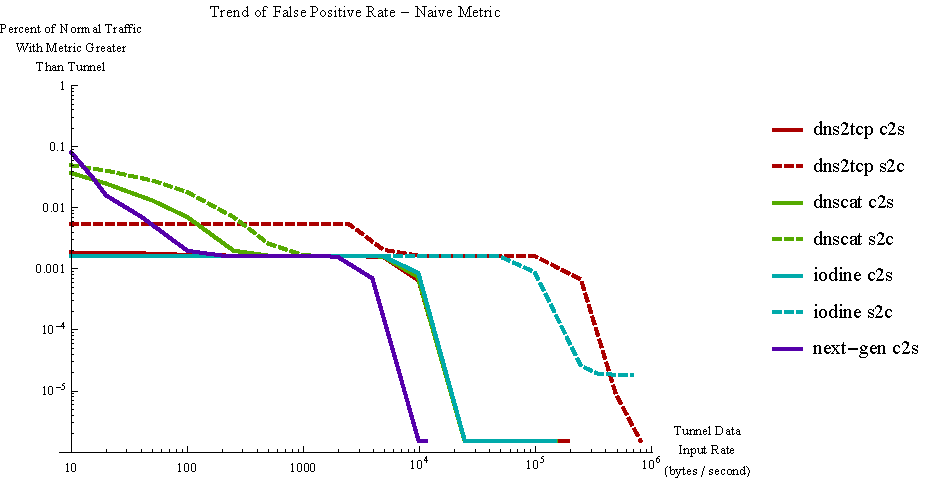
\includegraphics[width=\textwidth]{../figures/cnplot.pdf}
%%%\caption[Trend of False Positive Rate for Tunnels by Throughput - Naive 
%%%Metric]{Trend of False Positive Rate for Tunnels by Throughput - Naive Metric}
%%%\label{cnplot}
%%%\end{figure}
%%%
%%%\begin{figure}[h]
%%%\centering
%%%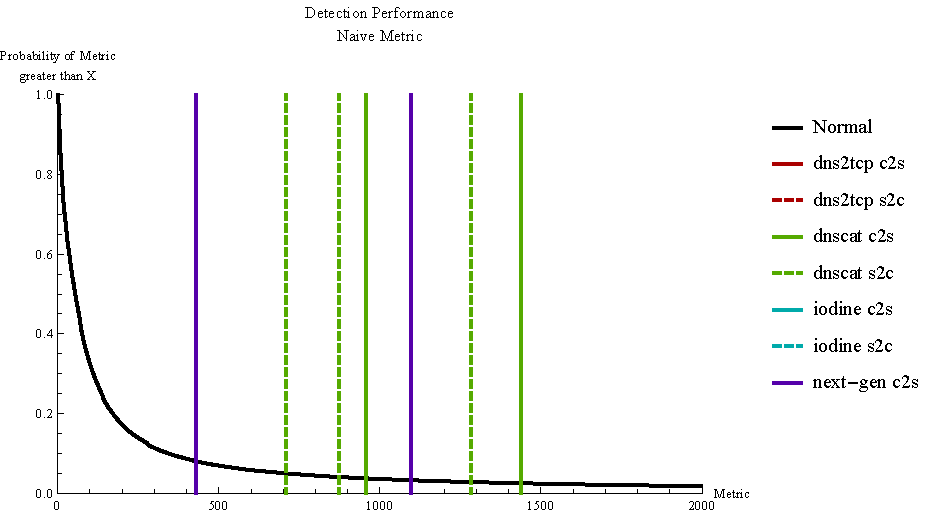
\includegraphics[width=\textwidth]{../figures/mpnv.pdf}
%%%\caption[Tunnel Detection Performance - Naive Metric]{Tunnel Detection 
%%%Performance - Naive Metric}
%%%\label{mpnv}
%%%\end{figure}

\begin{figure}[h]
\centering
\subfigure[Trend of False Positive Rate for Tunnels by Throughput - Naive Metric]{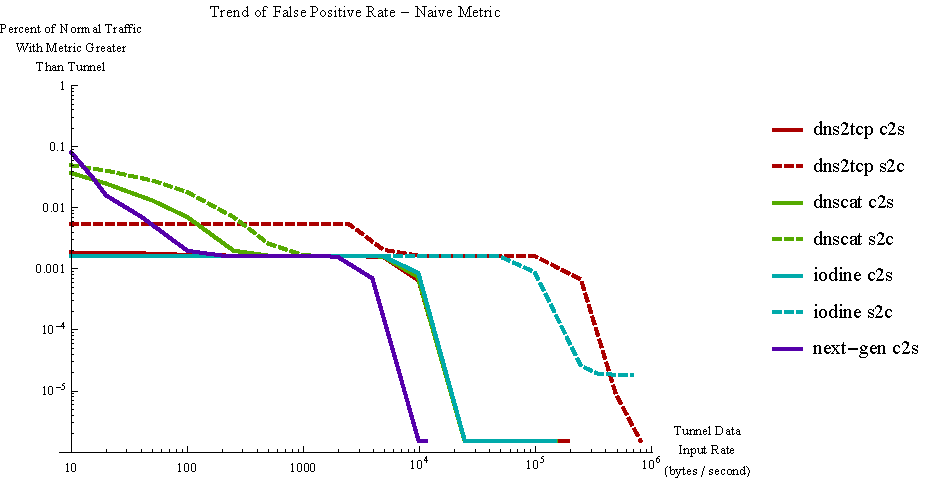
\includegraphics[width=0.48\textwidth]{../figures/cnplot.pdf}\label{cnplot}}
\subfigure[Tunnel Detection Performance - Naive Metric]{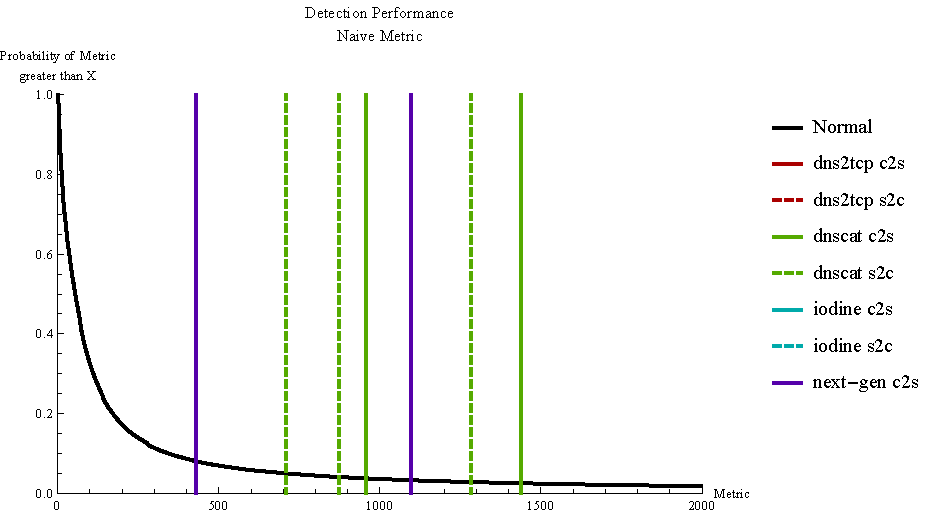
\includegraphics[width=0.48\textwidth]{../figures/mpnv.pdf}\label{mpnv}}
\caption{Tunnel detection performance for the naive approach.}
\label{mpn}
\end{figure}

%%%Figure \ref{mpnv} shows the performance of the naive metric, with markers
%%%visible for the next-gen and DNSCat tunnels. The lowest marker belongs to the
%%%next-gen tunnel, and has a false positive rate of 0.0799815, followed by a
%%%DNSCat server-to-client transfer with a rate of 0.0496253. Iodine's
%%%client-to-server transfers are the most easily detectable with its lowest false
%%%positive rate at 0.00164529 indicating a very low ambiguity when classifying its
%%%traffic.
%%%
The naive method, due to the nature of the the capture involving (relatively)
very few duplicate queries, performs quite well overall even on the next-gen
tunnel traffic. Figure \ref{cnplot} shows the trends of the false positive rate
for the tunnelling applications as a function of the data throughput. The lack
of duplication in the DNS queries and its impacts were discussed in section
\ref{dns-caching} in greater detail.

%%%\begin{figure}[h]
%%%\centering
%%%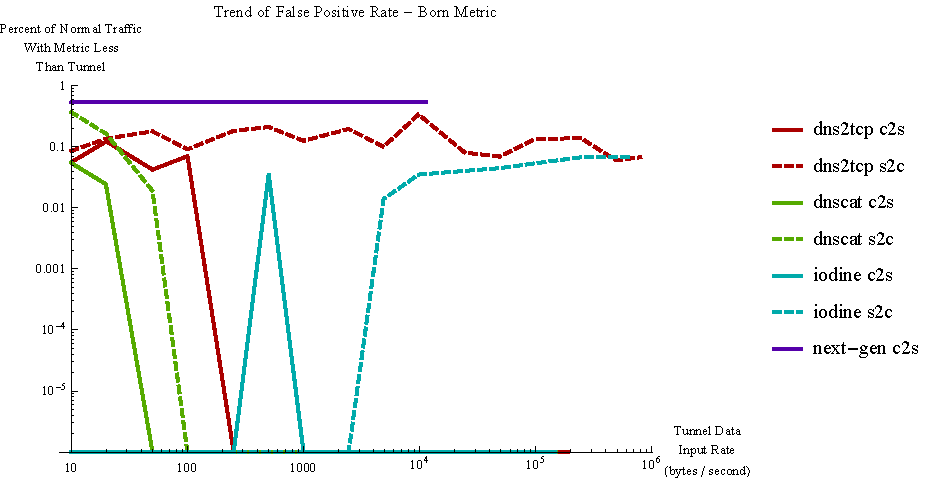
\includegraphics[width=\textwidth]{../figures/cbplot.pdf}
%%%\caption[Trend of False Positive Rate for Tunnels by Throughput - Born's 
%%%Metric]{Trend of False Positive Rate for Tunnels by Throughput - Born's Metric}
%%%\label{cbplot}
%%%\end{figure}
%%%
%%%\begin{figure}[h]
%%%\centering
%%%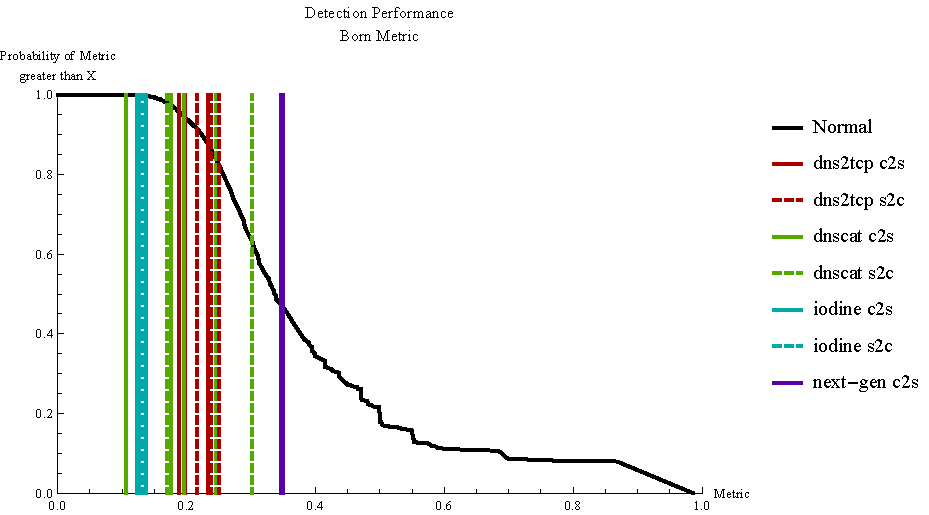
\includegraphics[width=\textwidth]{../figures/mpbv.pdf}
%%%\caption[Tunnel Detection Performance - Born's Metric]{Tunnel Detection 
%%%Performance - Born's Metric}
%%%\label{mpbv}
%%%\end{figure}

\begin{figure}[h]
\centering
\subfigure[Trend of False Positive Rate for Tunnels by Throughput - Born's Metric]{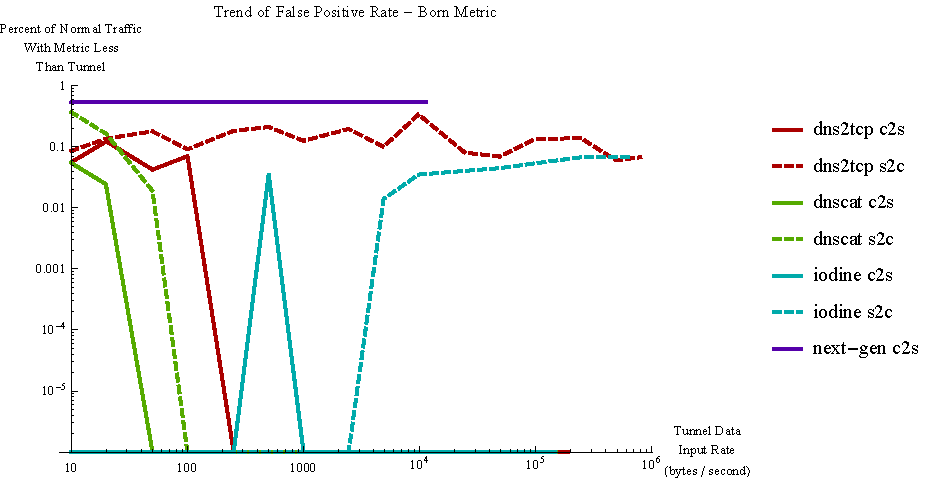
\includegraphics[width=0.48\textwidth]{../figures/cbplot.pdf}\label{cbplot}}
\subfigure[Tunnel Detection Performance - Born's Metric]{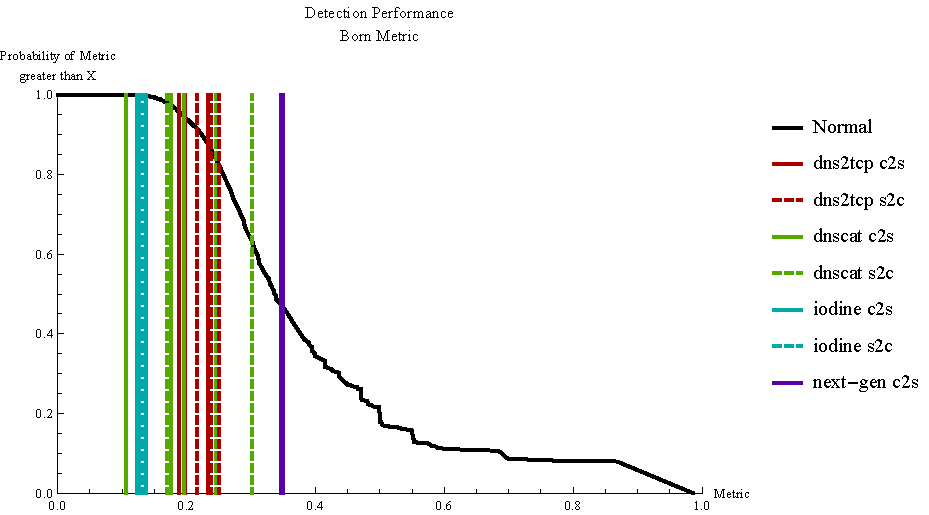
\includegraphics[width=0.48\textwidth]{../figures/mpbv.pdf}\label{mpbv}}
\caption{Tunnel detection performance for Born's approach.}
\label{mpb}
\end{figure}

%%%Figure \ref{mpbv} shows the performance of Born's metric with almost all markers
%%%visible clustered near the smaller metric values. Since the implementation of
%%%Born's metric produces smaller metrics for tunnels, the highest values are the
%%%ones of interest. The highest false positive rate of 0.529347 occurs for the
%%%next-gen tunnels. It is not easily seen in the plot, but all sixteen (one for
%%%each target throughput) of the next-gen tunnel markers are superimposed on each
%%%other at that value. This is due to how the tunnel was implemented for the
%%%proof-of-concept, as all traffic generated very closely conforms to a specified
%%%distribution. This distribution produces a particular metric under the
%%%implementation of Born's approach, independent of the amount of throughput. The
%%%next-gen tunnel markers are followed by the DNSCat server-to-client marker with
%%%a false positive rate of 0.367036. Similarly to the naive metric, Iodine's
%%%client-to-server tunnel was the most easily detected tunnel with the lowest
%%%throughput samples achieving a rate of no more than 0.00133572.
%%%
%%%It is easily seen that Born's metric will not be able to identify the next-gen
%%%tunnel with any reasonable certainty due to the ambiguity caused by the tunnel's
%%%traffic generating metrics very near to the median of real-world traffic. It is
%%%possible to augment the next-gen tunnel to adhere less tightly to a given
%%%distribution in order to spread its metrics over a wider range surrounding the
%%%median, further increasing the difficulty of detection. Figure \ref{cbplot}
%%%shows the trends of the crossing values for the tunnelling applications as a
%%%function of the data throughput.
%%
%%%\begin{figure}[h]
%%%\centering
%%%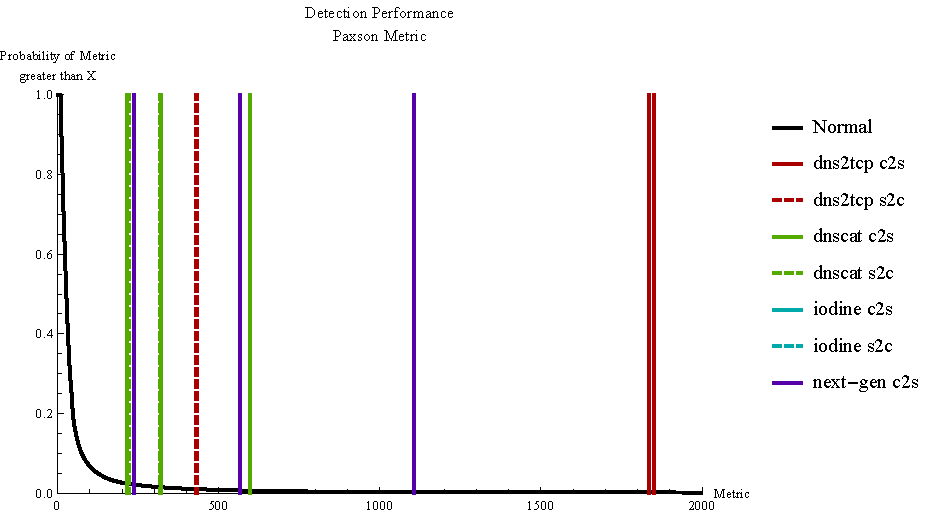
\includegraphics[width=\textwidth]{../figures/mppv.pdf}
%%%\caption[Tunnel Detection Performance - Paxson's Metric]{This visualizes the
%%%ability of Paxson's metric to discern a DNS tunnel from normal DNS traffic.}
%%%\label{mppv}
%%%\end{figure}
%%
%%%\begin{figure}[h]
%%%\centering
%%%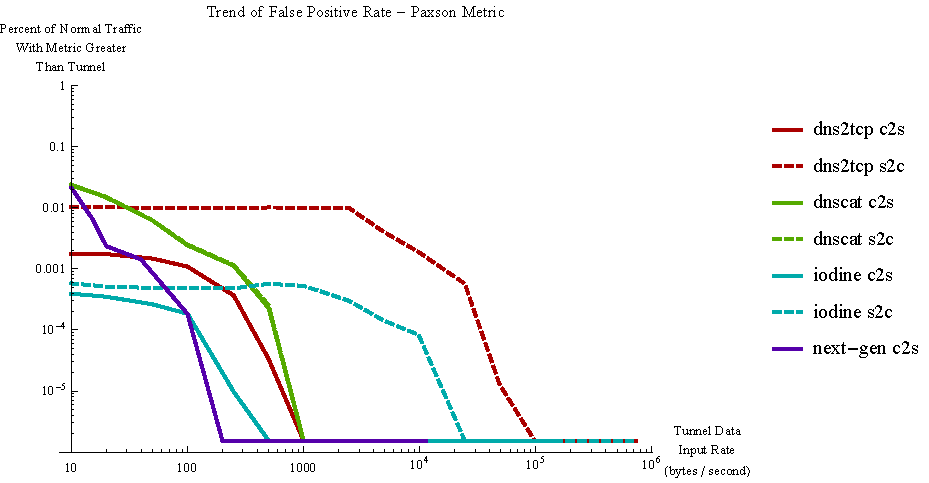
\includegraphics[width=\textwidth]{../figures/cpplot.pdf}
%%%\caption[Trend of False Positive Rate for Tunnels by Throughput - Paxson's 
%%%Metric]{Trend of False Positive Rate for Tunnels by Throughput - Paxson's 
%%%Metric}
%%%\label{cpplot}
%%%\end{figure}
%%%
%%%\begin{figure}[h]
%%%\centering
%%%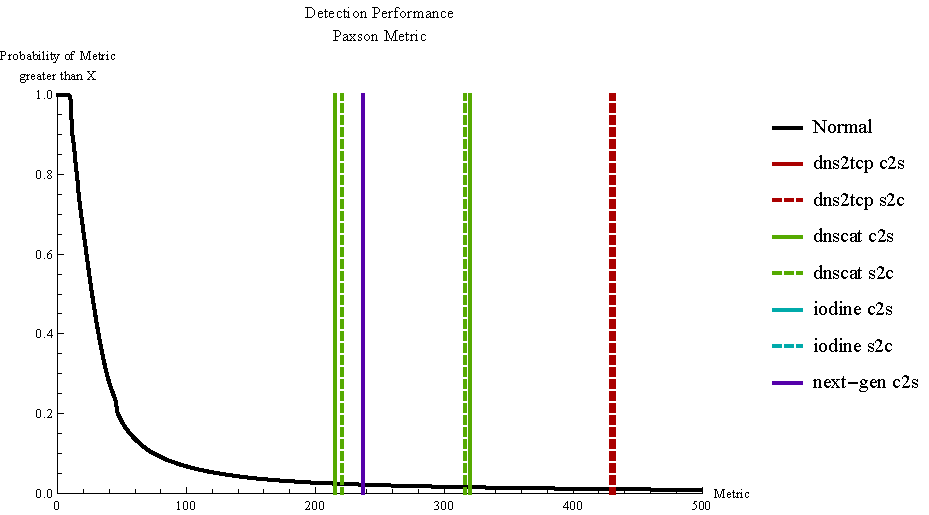
\includegraphics[width=\textwidth]{../figures/mppv-500.pdf}
%%%%\caption[Tunnel Detection Performance - Naive Metric (Truncated View)]{A cropped
%%%%plot of figure \ref{mppv} that offers more resolution in the smaller metric
%%%%ranges.}
%%%%\label{mppv-500}
%%%\caption[Tunnel Detection Performance - Paxson's Metric]{Tunnel Detection 
%%%Performance - Paxson's Metric}
%%%\label{mppv}
%%%\end{figure}

\begin{figure}[h]
\centering
\subfigure[Trend of False Positive Rate for Tunnels by Throughput - Paxson's Metric]{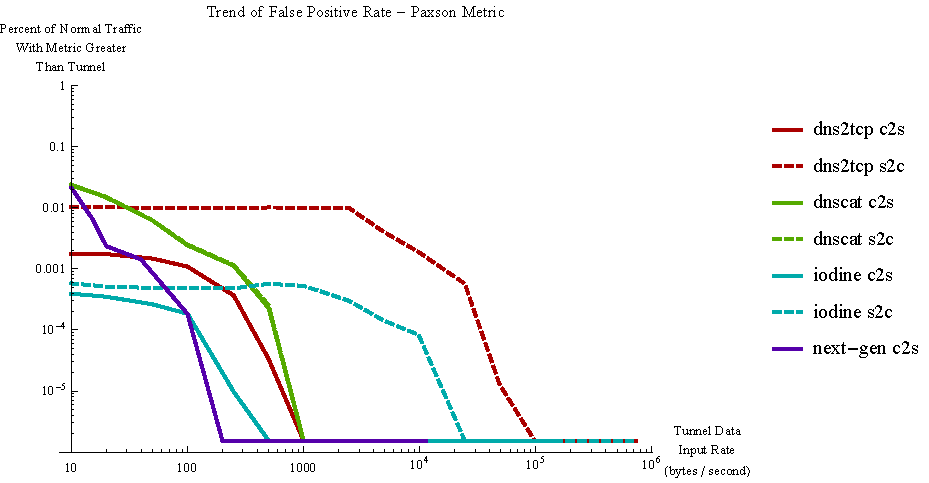
\includegraphics[width=0.48\textwidth]{../figures/cpplot.pdf}\label{cpplot}}
\subfigure[Tunnel Detection Performance - Paxson's Metric]{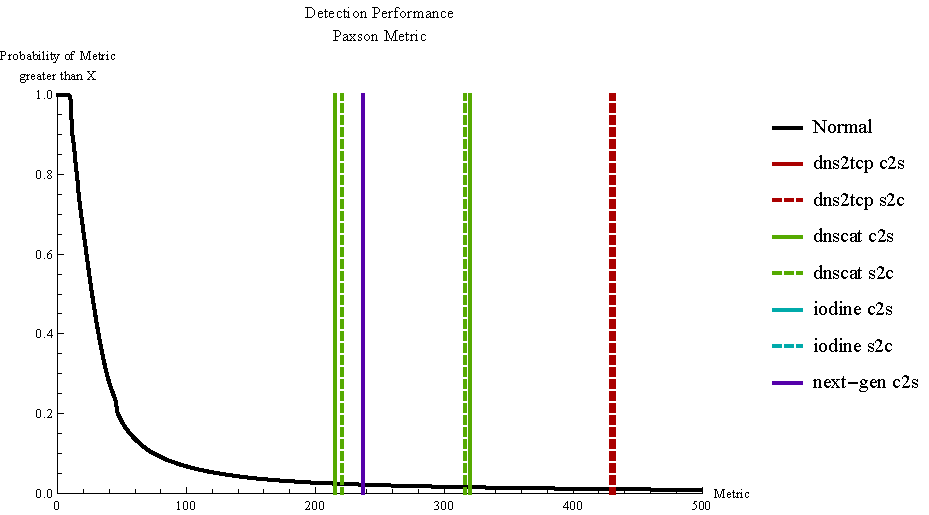
\includegraphics[width=0.48\textwidth]{../figures/mppv-500.pdf}\label{mppv}}
\caption{Tunnel detection performance for Paxson's approach.}
\label{mpp}
\end{figure}

%%%Figure \ref{mppv} shows the performance of Paxson's metric similarly to the plot
%%%shown for the naive method. The lowest metric is shown by the DNSCat
%%%client-to-server transfer with a false positive rate of 0.0239753 followed very closely by
%%%DNSCat's server-to-client transfer with a rate of 0.0232046. The next-gen tunnel
%%%produces a false positive rate of 0.0212873 and again Iodine is the most easily
%%%detected with its client-to-server transfers producing false positives at a
%%%proportion no larger than 0.00392552.
%%%
%%%As is expected, Paxson's method shows considerable improvement over both
%%%Born's approach and the naive method in terms of ambiguity of tunnel detection.
%%%Figure \ref{cpplot} shows the trends of the false positive rates for the
%%%tunnelling applications as a function of the data throughput.

%%%\begin{figure}[h]
%%%\centering
%%%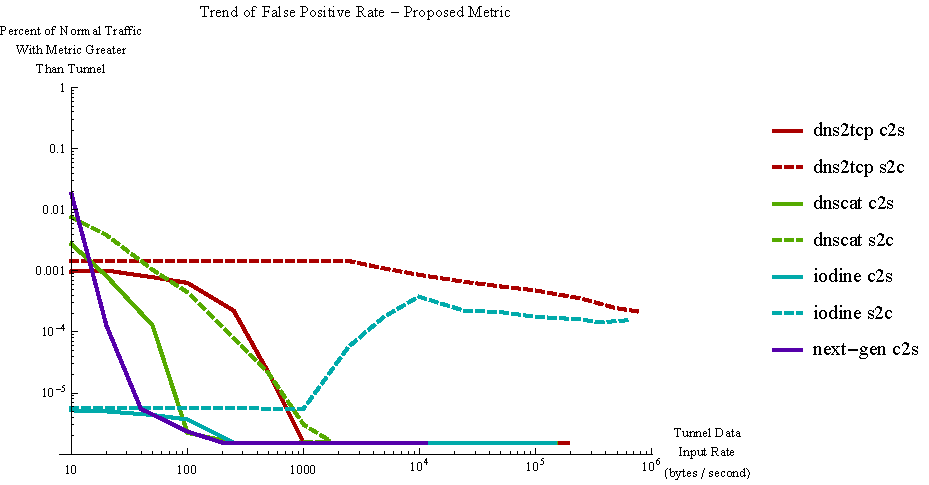
\includegraphics[width=\textwidth]{../figures/chplot.pdf}
%%%\caption[Trend of False Positive Rate for Tunnels by Throughput - Proposed Metric]{Trend
%%% of False Positive Rate for Tunnels by Throughput - Proposed Metric}
%%%\label{chplot}
%%%\end{figure}
%%%
%%%%\begin{figure}[h]
%%%%\centering
%%%%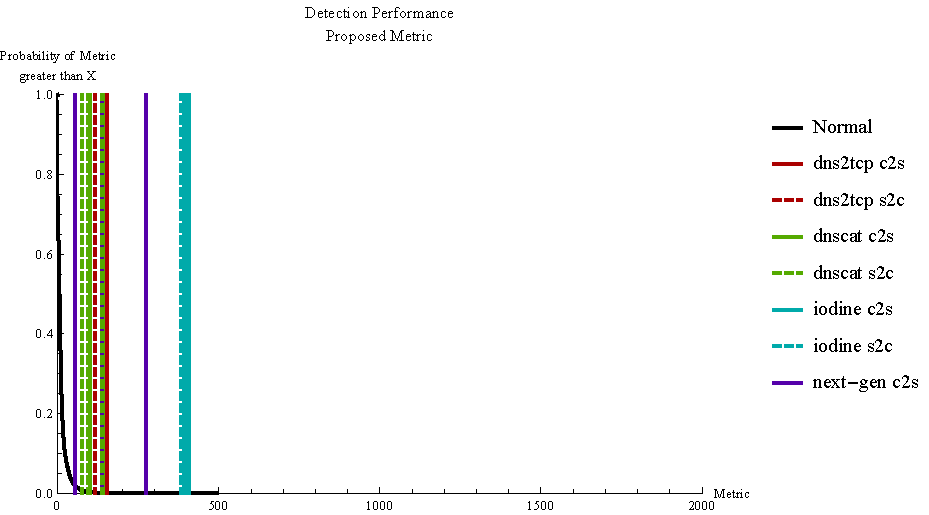
\includegraphics[width=\textwidth]{../figures/mphv.pdf}
%%%%\caption[Tunnel Detection Performance - Proposed Metric]{This visualizes the
%%%%ability of the proposed metric to discern a DNS tunnel from normal DNS traffic.}
%%%%\label{mphv}
%%%%\end{figure}
%%%\begin{figure}[h]
%%%\centering
%%%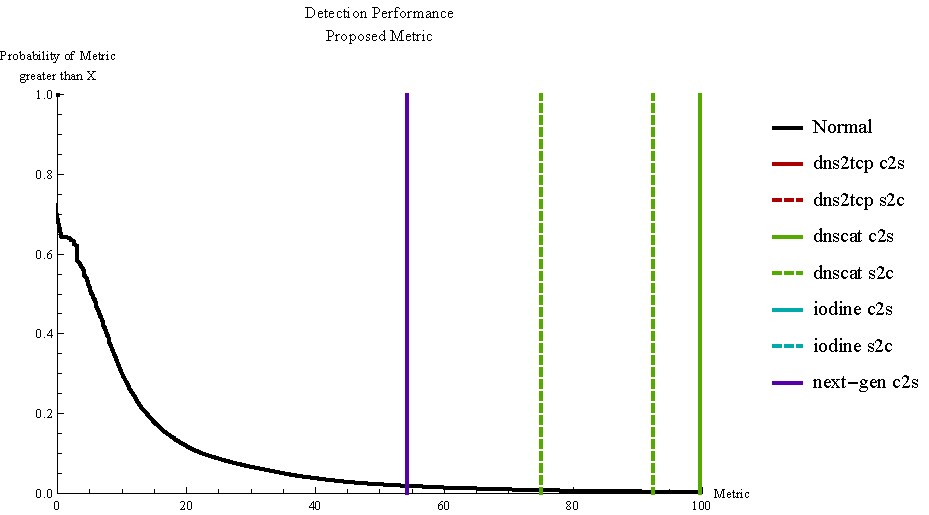
\includegraphics[width=\textwidth]{../figures/mphv-100.pdf}
%%%%\caption[Tunnel Detection Performance - Proposed Metric (Truncated View)]{A
%%%%cropped plot of figure \ref{mphv} that offers more resolution in the smaller
%%%%metric ranges.}
%%%%\label{mphv-100}
%%%\caption[Tunnel Detection Performance - Proposed Metric]{Tunnel Detection 
%%%Performance - Proposed Metric}
%%%\label{mphv}
%%%\end{figure}

\begin{figure}[h]
\centering
\subfigure[Trend of False Positive Rate for Tunnels by Throughput - Proposed Metric]{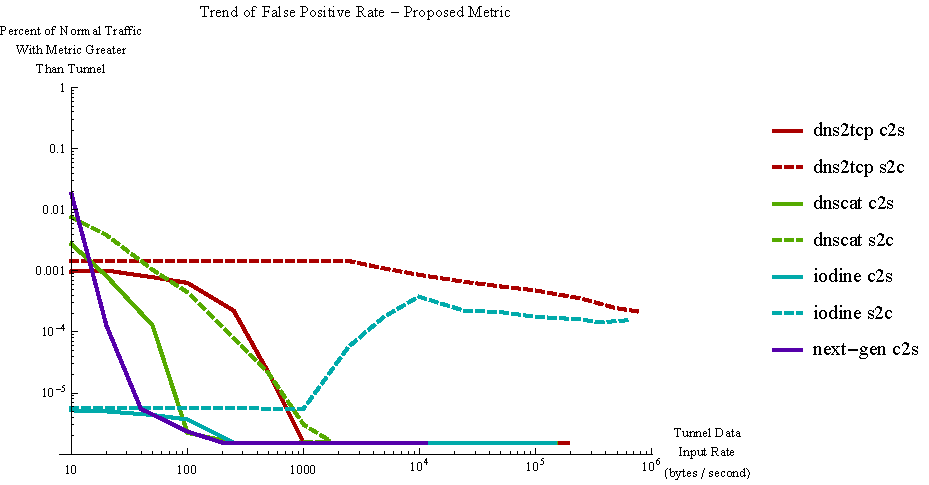
\includegraphics[width=0.48\textwidth]{../figures/chplot.pdf}\label{chplot}}
\subfigure[Tunnel Detection Performance - Proposed Metric]{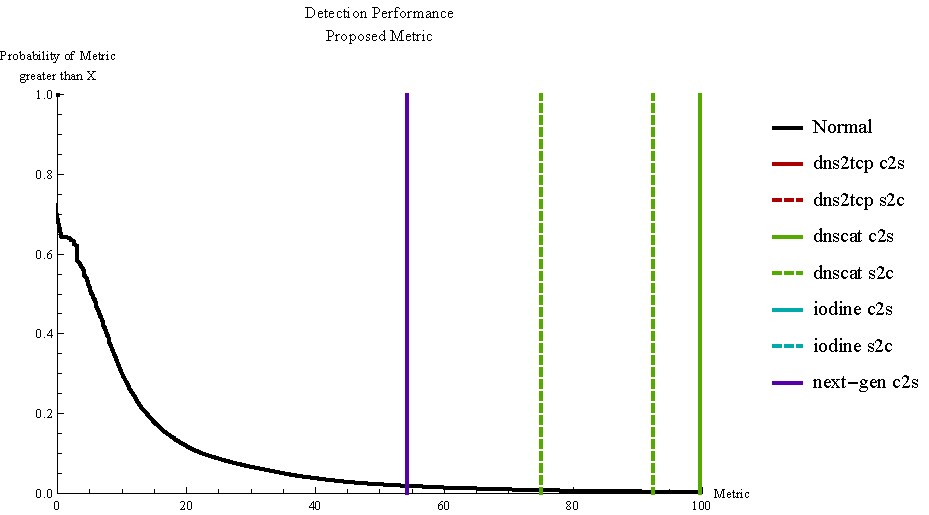
\includegraphics[width=0.48\textwidth]{../figures/mphv-100.pdf}\label{mphv}}
\caption{Tunnel detection performance for our approach.}
\label{mph}
\end{figure}

%\begin{figure}[h]
%\centering
%\subfigure[Trend of False Positive Rate for Tunnels by Throughput - Naive Metric]{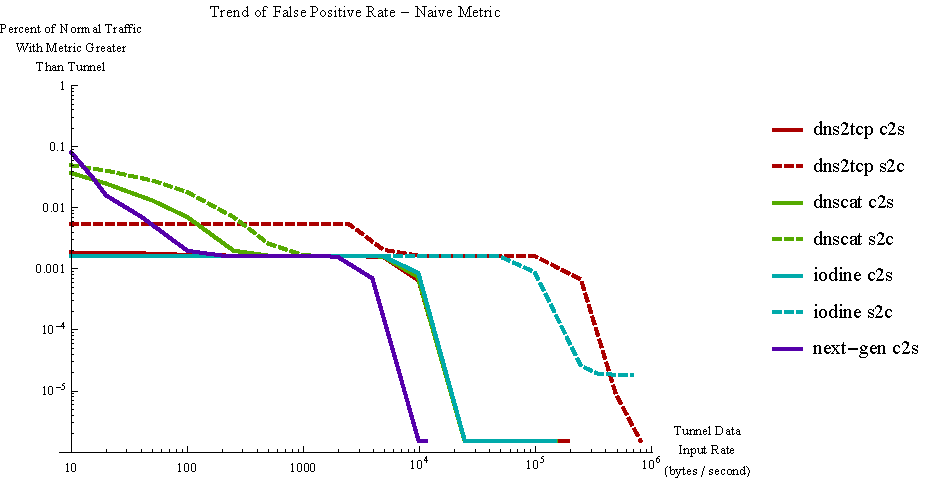
\includegraphics[width=0.48\textwidth]{../figures/cnplot.pdf}\label{cnplot}}
%\subfigure[Tunnel Detection Performance - Naive Metric]{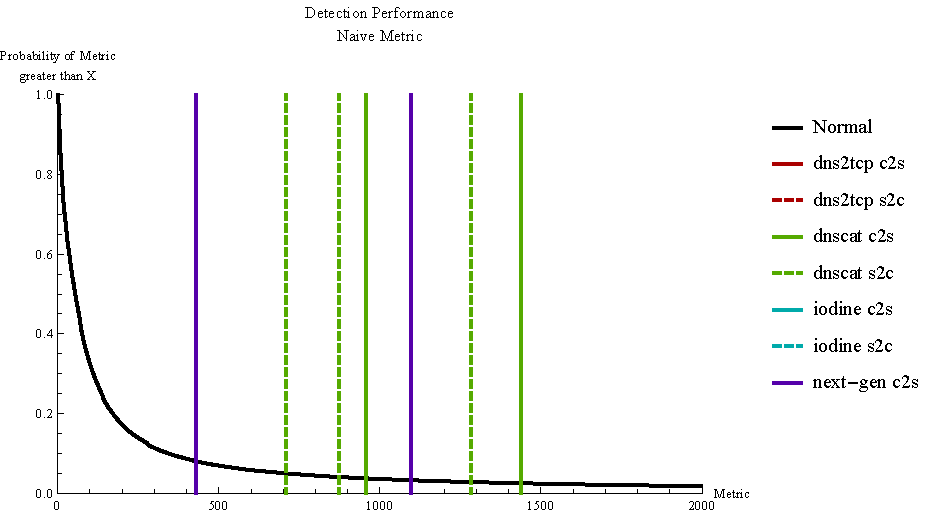
\includegraphics[width=0.48\textwidth]{../figures/mpnv.pdf}\label{mpnv}}
%
%\subfigure[Trend of False Positive Rate for Tunnels by Throughput - Born's Metric]{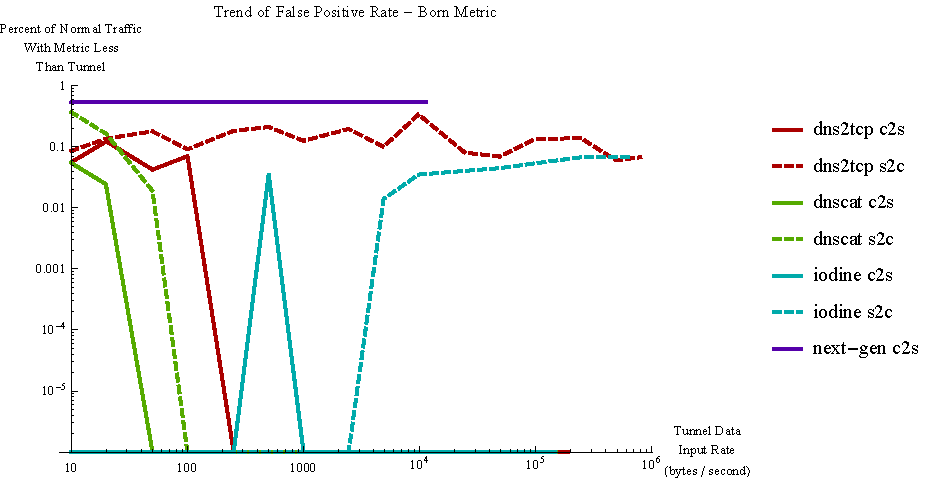
\includegraphics[width=0.48\textwidth]{../figures/cbplot.pdf}\label{cbplot}}
%\subfigure[Tunnel Detection Performance - Born's Metric]{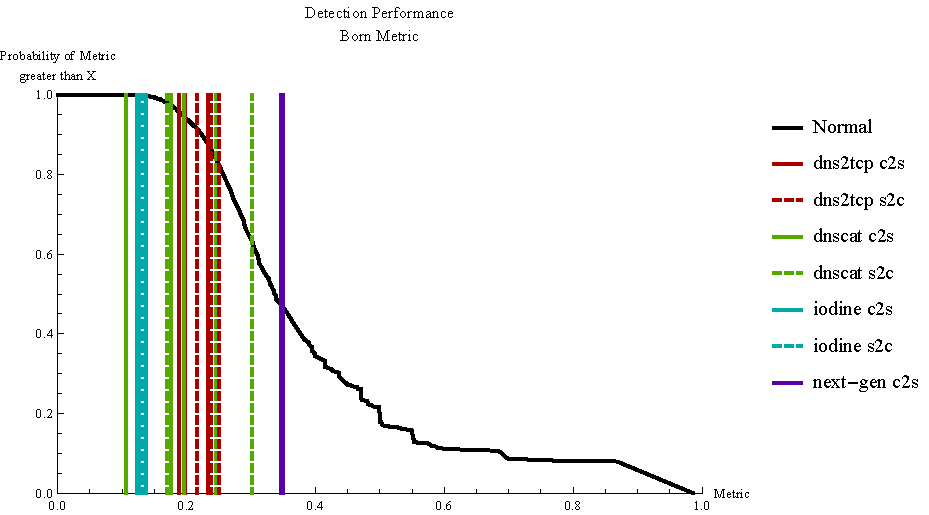
\includegraphics[width=0.48\textwidth]{../figures/mpbv.pdf}\label{mpbv}}
%
%\subfigure[Trend of False Positive Rate for Tunnels by Throughput - Paxson's Metric]{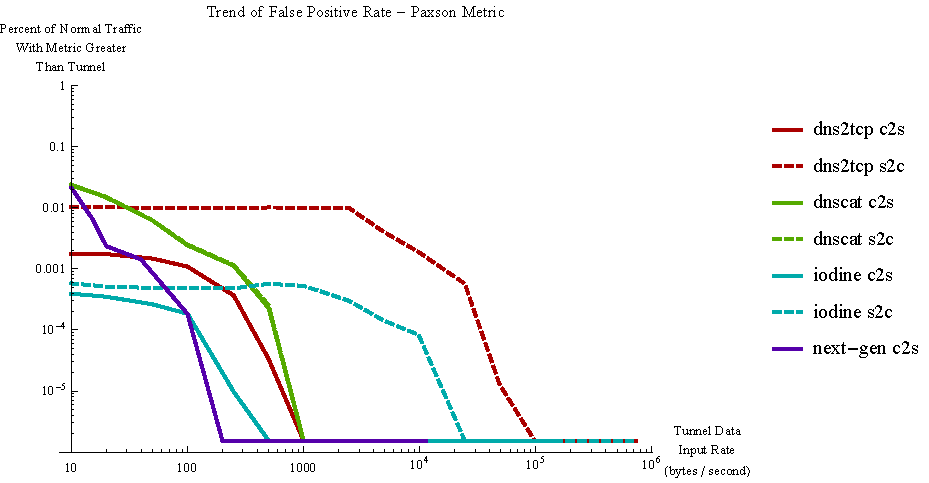
\includegraphics[width=0.48\textwidth]{../figures/cpplot.pdf}\label{cpplot}}
%\subfigure[Tunnel Detection Performance - Paxson's Metric]{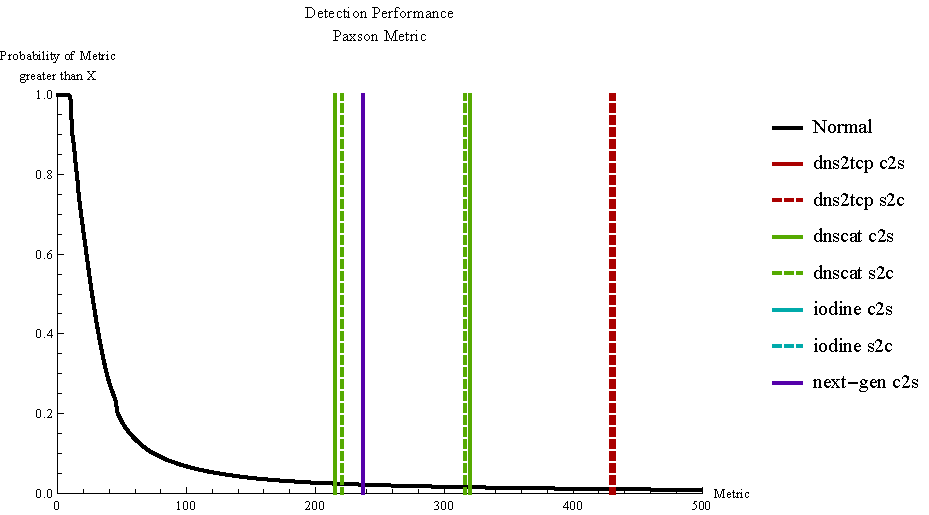
\includegraphics[width=0.48\textwidth]{../figures/mppv-500.pdf}\label{mppv}}
%
%\subfigure[Trend of False Positive Rate for Tunnels by Throughput - Proposed Metric]{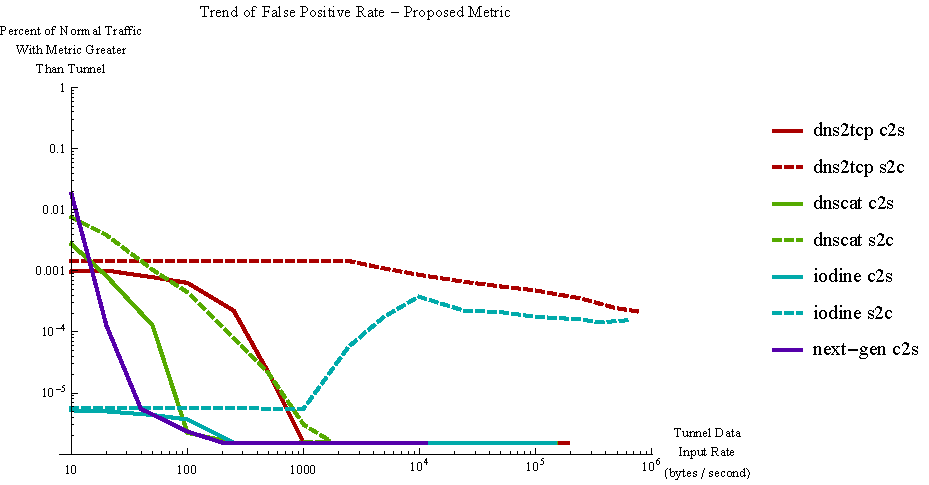
\includegraphics[width=0.48\textwidth]{../figures/chplot.pdf}\label{chplot}}
%\subfigure[Tunnel Detection Performance - Proposed Metric]{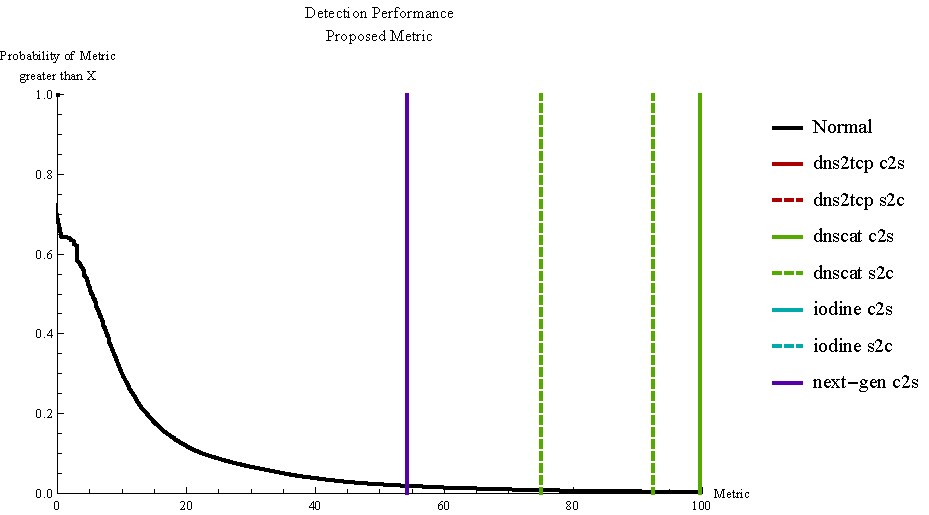
\includegraphics[width=0.48\textwidth]{../figures/mphv-100.pdf}\label{mphv}}
%\caption{Tunnel detection performance for detection approaches}
%\label{mpv}
%\end{figure}

%%%Figure \ref{mphv} shows the performance of the proposed metric in a fashion
%%%similar to the naive method and for Paxson's method. The highest false positive
%%%rate encountered is from the next-gen tunnel at 0.0184927. This is followed by
%%%two of the samples generated by the DNSCat server-to-client transfers, the first
%%%of which produced a false positive rate of 0.00751152. As has been the case for all
%%%metrics thus far, Iodine is the most easily detected tunnel generating
%%%proportions of false positives for its lowest throughput client-to-server and
%%%server-to-client transmissions of no more than $5.19129\times10^{-6}$ and
%%%$5.73392\times10^{-6}$ respectively.

\subsection{Specificity and Ambiguity of Tunnel Classification}
\label{detection-perf-cert}

It is possible to simplify the above plots and figures into a single chart that
plots the minimum detection specificity observed for each method and each
tunnelling application. The following charts only consider the certainty of
detecting the tunnel in which the method is least certain. By comparing the
methods in their most hostile scenarios more substantial distinctions can be
observed with clearer separation between the best two methods.
%%%In all cases,
%%%this corresponded to one of the tunnelling applications at the ten bytes per
%%%second throughput level, which demonstrates the effectiveness of these methods
%%%to solve the \emph{needle-in-a-haystack} problem of low throughput DNS tunnels
%%%on a very busy network link.
%%
%%%%\begin{figure}[h]
%%%%\centering
%%%%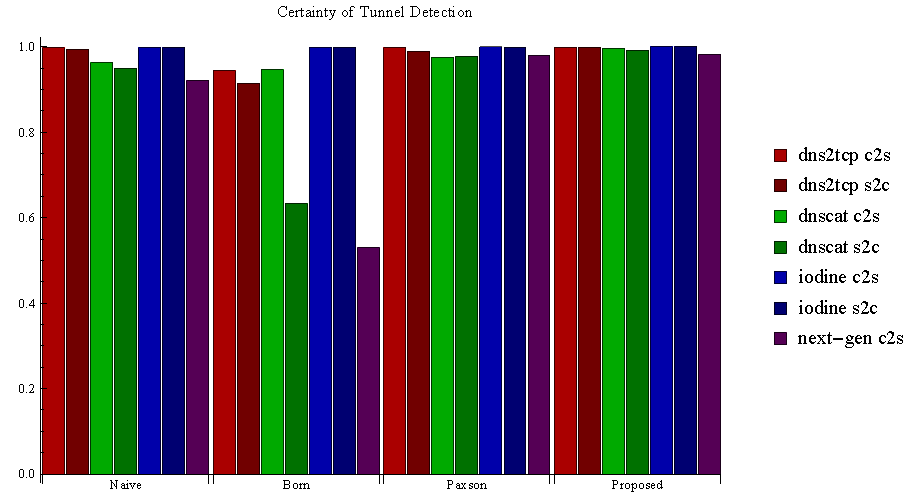
\includegraphics[width=\textwidth]{../figures/cplot.pdf}
%%%%\caption[Chart of Specificity of Detection by Tunnel Application and Detection
%%%%Method]{Comparison of the specificity of classification of a tunnel against
%%%%real-world traffic for the least certain tunnel in each detection scenario
%%%%(method/application pair).}
%%%%\label{cplot}
%%%%\end{figure}

\begin{figure}[h]
\centering
\subfigure[Certainty of detection]{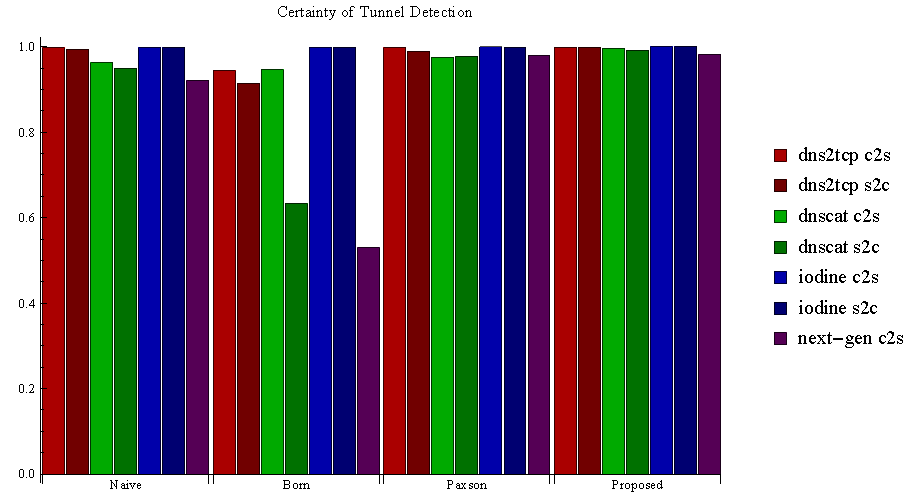
\includegraphics[width=0.48\textwidth]{../figures/cplot.pdf}\label{cplot}}
\subfigure[Certainty of detection - 0.80 to 1.00]{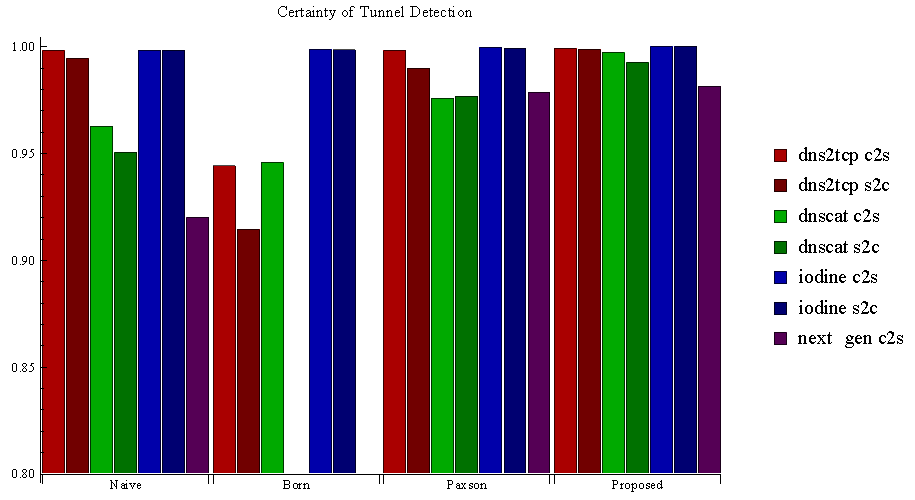
\includegraphics[width=0.48\textwidth]{../figures/cplot2.pdf}\label{cplot80}}
\caption{Certainty of tunnel detection by detection method.}
\end{figure}

\begin{figure}[h]
\centering
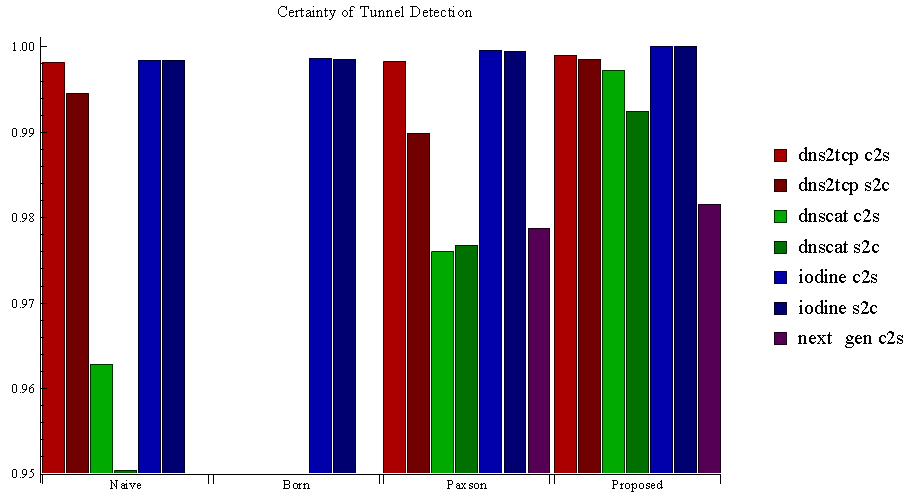
\includegraphics[width=\textwidth]{../figures/cplot3.pdf}
\caption[Chart of Specificity of Detection by Tunnel Application and Detection
Method]{Comparison of the specificity of classification of a tunnel against
real-world traffic for the least certain tunnel in each detection scenario
(method/application pair).}
\label{cplot95}
\end{figure}

%Figure \ref{cplot} shows the specificities of each method for each tunnelling
%application, in the interval $[0,1]$. Observe the extremely
%low certainty of Born's metric on two tunnelling applications (next-gen and
%DNSCat's server-to-client), with lacklustre performances for DNSCat's
%client-to-server and both DNS2TCP transfer directions. The only tunnelling
%application that Born's method reliably picks out is Iodine, however as was
%shown earlier Iodine is by far the most easily distinguished tunnel by a large
%margin for all detection methods. The naive and proposed methods as well as
%Paxson's method perform similarly with differences that are not easily
%distinguished in this chart.

%\begin{figure}[h]
%\centering
%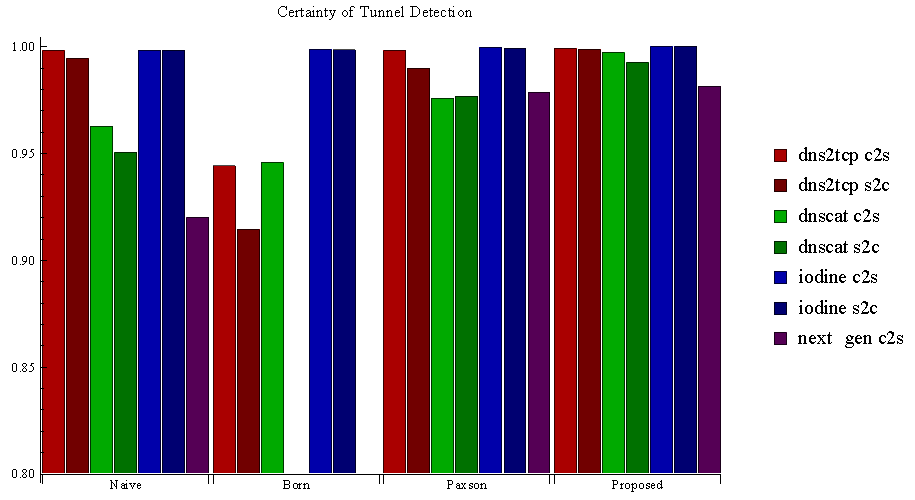
\includegraphics[width=\textwidth]{../figures/cplot2.pdf}
%\caption[Chart of Certainty of Detection by Tunnel Application and Detection
%Method - 0.80 to 1.00]{Figure \ref{cplot} replotted with a reduced range to
%accentuate small differences.}
%\label{cplot80}
%\end{figure}

Figure \ref{cplot80} shows the same data as in Fig. \ref{cplot} with a
restricted range spanning the interval $[0.80,1.00]$ as opposed to $[0,1]$. This
restricted charting range makes the the differences between the top performing
methods more easily visible.
%In this chart, it is easily seen that the naive
%method outperforms Born's method in all except the Iodine case. The Iodine
%performance differences are not easily visible due to the very close values. The
%naive method has a certainty of 0.998355 for both transfer directions while
%Born's method has certainties of 0.998664 and 0.998512 for the client-to-server
%and server-to-client directions respectively. The differences, on the order of
%0.0003, are not visible in the charts. The performance of the proposed method
%and Paxson's method relative to the naive method is clearly visible in this
%chart.

%\begin{figure}[h]
%\centering
%\includegraphics[width=\textwidth]{../figures/cplot3.pdf}
%\caption[Chart of Certainty of Detection by Tunnel Application and Detection
%Method - 0.95 to 1.00]{Figure \ref{cplot} replotted with a further reduced range to
%accentuate \emph{very} small differences.}
%\label{cplot95}
%\end{figure}

The differences between Paxson's method and our method are visible,
but an additional chart further accentuating them is instructive and
is shown in figure \ref{cplot95}. In this final chart which shows a
range of certainties in the interval $[0.95,1.00]$, the differences
between the two methods are clearly visible, with our approach
achieving a higher certainty in every detection scenario.

\subsection{Tunnel Detection Performance Conclusion}
It is visible from the detailed plots in Sect. \ref{detection-perf}
and \ref{detection-perf-cert} that our method is superior to its peers
in its ability to detect tunnels with certainty in excess of ninety
eight percent.  This extremely high detection rate is achieved within
a very short time scale and with very low tunnel throughput.

%% In this work, a new method of detecting DNS tunnels was proposed, described, and
%% evaluated.
%% %The existing landscape of detection methods was summarized (section
%% %\ref{litreview}) and a gap identified indicating a need for a new method
%% %(section \ref{methodreqs}) that has both high processing performance on
%% %commodity hardware, and robust tunnel detection. A prototypical next-gen tunnel
%% %application was postulated and simulated in order to present a more difficult detection
%% %task during evaluation alongside existing tunnel applications (section
%% %\ref{test-existing}). Several detection methods from the literature as well as
%% %the proposed method were selected (section \ref{chosen-methods}) and implemented
%% %on a common framework. The implemented methods
%% %were tested for processing performance (section \ref{processing-perf}) and
%% %tunnel detection performance on a large sample of real world DNS traffic as well
%% %as existing and next-gen tunnelling application data (section
%% %\ref{chap-evaluation}).
%% As is shown in the relevant sections, the proposed method outperforms its peers
%% in both processing performance and tunnel detection in almost every situation by
%% a measurable and often considerable margin.
%% %When compared to its peers from literature, the performance improvement over
%% %Paxson's approach on real-world data is approximately 25\% while a speedup of
%% %almost 100\% is observed when processing tunnel data under the Cython
%% %interpreter. The margins are similar under PyPy, with the primary difference
%% %being that the proposed method is nearly double the performance of Paxson's
%% %approach on both real world and tunnel application data. Born's approach is able
%% %to narrow the gap on tunnel data to only approximately a 50\% improvement, while
%% %the gap on real-world data increases to about 30\%. Under PyPy however, the
%% %performance of the proposed method and Born's method become very similar with
%% %gaps less than 10\%.
%% %
%% %Examining tunnel detection performance shows additional benefits to the proposed
%% %method. Born's method shows very poor performance, as expected, when faced with
%% %the next-gen tunnel, with a less drastic performance hit shown on other
%% %tunnelling software. In all cases the proposed, as well as Paxson's, approach
%% %out-perform Born's method by a considerable margin in false-positive rates. The
%% %proposed approach reduces the false positive rate by almost 98\% when compared
%% %to Born's approach. When comparing Paxson's approach with the proposed
%% %approach, the proposed approach reduces the number of false positives by up to
%% %nearly 90\% in the best case, with an average reduction of 70\%.
%% %
%% %The exception is the naive method which outperforms the proposed method in
%% %processing performance by approximately fifty percent at the expense of
%% %detection performance, with the proposed approach reducing the false positive
%% %rate by 82\%. As was mentioned in Sect. \ref{dns-caching} however,
%% %the naive method's detection performance is only as good as it is in this case
%% %due to the lack of duplication of DNS queries.
%% Recall that the improvements demonstrated of our approach are measured
%% in a highly pessimistic detection scenario, with false-positive rates
%% rapidly dropping below $10^{-6}$ as throughput increases.

%% The end product of these results is a contribution to the field
%% composed of a new detection method with superior processing and
%% detection performance.
%% %The new
%% %detection method falls short of matching the naive method's processing
%% %performance in many situations with the trade off of far superior detection
%% %performance in the general case.

\section{Conclusion and Future Work}
\label{conclusion}
%The proposed method was shown to be highly effective in detecting the targeted
%network traffic with superior performance, outperforming existing methods in almost
%every scenario. In order for this to be of value, however, an adoption of this
%method into an existing commercial products or an implementation as a plugin for
%an existing security framework would be necessary.

This paper describes our entropy-based detection method for DNS
tunnels and shows through an empirical evaluation that our approach
provides better detection accuracy and faster processing than previous
approaches described in the literature. Our method works well not only
in artificial benchmark datasets, but also in difficult real-world
traffic. 

%We also show a method for encoding data such that it closely matches a
%desired character frequency distribution, which completely circumvents
%some current detection methods ***cite.

Future work includes implementing our method for Bro, Snort, Suricata
or other existing intrusion detection systems in order to improve the
ability of organizations to observe DNS tunnels in their
network. Partnership with, and adoption by, an existing industry
partner would aid in the spread and deployment of this technique in
enterprise and corporate environments.
%Due to the nature of
%computer security research, regardless of how valuable a contribution may be, unless
%there is deployment of the approach into real world environments it is unable
%to aid in securing the Internet.

\bibliography{../Reference/bibliography}

\end{document}
